% $Id: ESMF_usrdoc.tex,v 1.10 2003/04/09 17:08:28 cdeluca Exp $

\documentclass[]{article}

\usepackage{graphicx}
\usepackage{html}
\usepackage{times}
\usepackage[T1]{fontenc}

\textwidth 6.5in
\textheight 8.5in
\addtolength{\oddsidemargin}{-.75in}


\begin{document}

\bodytext{BGCOLOR=white LINK=#083194 VLINK=#21004A}

\begin{titlepage}

\begin{center}
{\Large Earth System Modeling Framework } \\
\vspace{.25in}
{\Large {\bf Earth System Modeling Framework User Guide}} \\
\vspace{.25in}
{\large {\it Release 1.0}}
\vspace{.5in}
\end{center}

\begin{latexonly}
\vspace{5.5in}
\begin{tabular}{p{5in}p{.9in}}
\hrulefill \\
\noindent {\bf NASA High Performance Computing and Communications Program} \\
\noindent Earth and Space Sciences Project \\
\noindent CAN 00-OES-01 \\
\noindent http://www.esmf.ucar.edu \\
\end{tabular}
\end{latexonly}

\end{titlepage}

\tableofcontents

\newpage

\setlength{\parskip}{2ex}
\setlength{\parindent}{0ex}

%\section{Introduction}

\section{Release Notes}

The purpose of ESMF v1.0 is to provide a first look at the ESMF
Application Programming Interface (API), and to demonstrate the viability 
of the ESMF architecture and implementation.  For this release, we have focused 
on implementing major architectural features and basic functionality.  The 
current performance characteristics and memory requirements of the software 
are unlikely to resemble those in later releases.  

We are relying on Earth system modelers to provide us with the feedback necessary 
to realize this goal.  Section \ref{sec:Support} of this document includes 
instructions on submitting comments on ESMF v1.0 to our development team.

Our next major release, ESMF v2.0, will occur in April 2004.  At that time, 
the {\it ESMF User's Guide} will be expanded to include a comprehensive section 
on how to adapt application codes for the framework, and support staff will be 
available to assist users with ESMF adoption.  We anticipate, but have 
not scheduled, other public releases and patches between now and ESMF v2.0.  
Our focus during this year will be on developing an easy to use, production-quality 
product.  

\section{What is the Earth System Modeling Framework?}

The Earth System Modeling Framework (ESMF) is a structured collection of 
software building blocks that can be used or customized to develop 
Earth system model components, and assemble them into applications.  
The simplest view of the ESMF is that it consists of an {\it infrastructure} 
of utilities and data structures for creating 
model components, and a {\it superstructure} for coupling them.  
User code sits between these two layers, making calls to the infrastructure
libraries beneath it and being scheduled and synchronized by the 
superstructure above it.  The configuration resembles a sandwich, as
shown in Figure~\ref{fig:TheESMFwich}.

The ESMF architecture is scalable, flexible paradigm for building highly 
complex climate, weather, and related applications from components such
as atmospheric models, land models, and data assimilation systems.  The 
ESMF is not a single master application into which all components must fit; 
rather it is a way of developing components so that they can be used 
in many different user-written applications.  Model components that adopt 
ESMF are usable in different contexts without code modification, and may be
incorporated into other ESMF-based modeling systems within the Earth 
science community.  In addition to high-level organization, ESMF provides 
a set of robust, portable, performance optimized libraries for regridding, 
data transfers, I/O, time management, and other common modeling functions.  
ESMF users may choose to extensively rewrite their codes to take advantage 
of the ESMF infrastructure, or they may decide to simply wrap user-written 
components in ESMF interfaces in order to adopt the ESMF architecture and 
utilize framework coupling services.

\section{The ESMF User's Guide}

This {\it ESMF User's Guide} will eventually serve as an introduction for the 
new ESMF user and as a reference for the experienced user.  Since ESMF 
Release 1.0 is the first public ESMF release, and is a prototype rather than 
a production-ready package, we assume you are a potential user interested in 
learning more about the ESMF software.  This edition of the {\it User's Guide} 
is designed to guide you through that process.  We strongly encourage you
to download the ESMF software and try running a demonstration program, 
{\tt ESMF\_COUPLED\_FLOW}, that illustrates both ESMF utilities and coupling
services.

The next two sections, \ref{sec:Support} and \ref{sec:Submission}, concern 
user support and how to submit comments on the ESMF system to our develoment 
team.  Section \ref{sec:QuickStart} contains a {\it Quick Start} guide that 
explains how to install the ESMF software and 
run the demonstration program.  Section \ref{sec:ArchOver} is an 
architectural overview that describes the framework's basic goals and features.The next few Sections, beginning with \ref~{sec:demo}, describe in detail
the {\tt ESMF\_COUPLED\_FLOW} demo application.    
More detail on ESMF structure and operation, such as a description of the 
directory structure and how to run the ESMF self-tests, is provided in Section 
\ref{sec:TechOver}.  Section \ref{sec:Adoption} looks ahead to the steps 
required to adapt a component for use with ESMF.  Finally, to help you become 
familiar with ESMF terminology, the last section in the {\it User's Guide} is 
a glossary.  

\begin{center}
\begin{figure}
\caption{Schematic of ESMF ``sandwich'' architecture. In this design the framework consists of two parts. An upper level
{\bf Superstructure} layer and a lower-level {\bf Infrastructure} layer. User code is sandwiched between these two layers.}
\label{fig:TheESMFwich}
\scalebox{1.0}{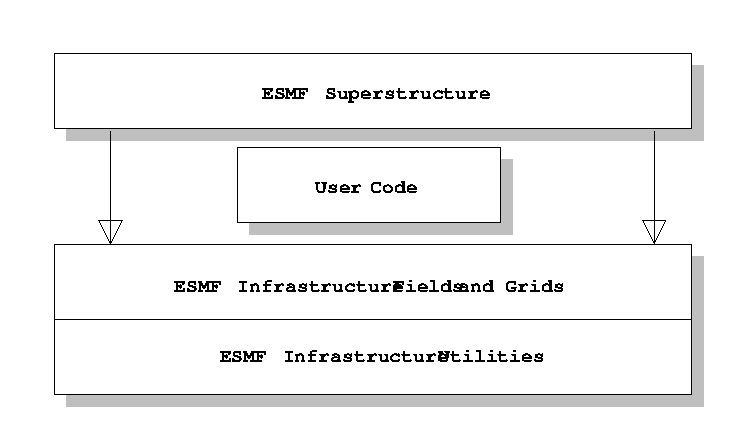
\includegraphics{esmfwich.EPS}}
\end{figure}
\end{center}


















%\section{ESMF Support and Contacts}
\section{User Support and Contact Information}

The ESMF team can provide assistance in running the demonstration 
at your site.  For user support, please contact \htmladdnormallink{esmf\_support@ucar.edu}
{mailto:esmf_support@ucar.edu}.  

More information on the ESMF project as a whole is available on the 
ESMF website, \htmladdnormallink{http://www.esmf.ucar.edu}{http://www.esmf.ucar.edu}.  
Comments on the ESMF API and architecture may be submitted to the ESMF development 
team on-line via the {\bf Development} link on the ESMF website.  The {\bf Development} 
link on the ESMF website also includes on-line forms for the submission of 
new requirements, if it seems that the current API does not satisfy the needs of 
your application.  We welcome input on any aspect of the ESMF project; general
questions and comments should be sent to \htmladdnormallink{esmf@ucar.edu}
{mailto:esmf@ucar.edu}.






\newpage
%\section{Quick Start}
\section{Quick Start}
\label{sec:QuickStart}

This section describes how to get the ESMF software, install it, 
and run a demonstration application.  More detailed information about 
setting up the ESMF, such as how to modify library paths in the 
makefiles and how to run diagnostic self-tests, can be found in 
Section \ref{sec:TechOver}.  

% $Id: ESMF_install.tex,v 1.22 2003/05/07 14:14:38 cdeluca Exp $

\subsection{ESMF Download Options}

Major releases of the ESMF software can be downloaded by following
the instructions on the 
the {\bf Downloads \& Documentation} page on the ESMF 
website, \htmladdnormallink{http://www.esmf.ucar.edu}{http://www.esmf.ucar.edu}.  There are two options for using the ESMF:

\begin{itemize}
\item Download a pre-built ESMF shared object library and
test applications for a particular platform.  If you choose
this approach, you can skip ahead to Section~\ref{UsingLibrary},
Using the ESMF.  
\item Download the full ESMF source code, and compile and link
the framework to any necessary system libraries.  This will
result in a shared object file (with a *.so extension)
that can be linked in with the user's code, or with the demo
{ESMF\_COUPLED\_FLOW} executable.  In this case you will need
to follow all the instructions in subsequent sections of the 
{\it Quick Start} guide, beginning with Section~\ref{InstallProcedures},
Installation.
\end{itemize}

You may find it necessary to build the ESMF yourself
if we do not offer a shared object library for the current
version of your compiler.  The compiler versions that we offer
shared objects for are noted on the download web page.

\subsection{Installation}
\label{InstallProcedures}

% $Id: ESMF_systemreq.tex,v 1.2 2004/06/22 14:17:44 nscollins Exp $

\subsubsection{System Requirements}
\label{sec:systemreq}

The following compilers and utilities are required for compiling and 
linking the ESMF software:
\begin{itemize}
\item a Fortran90 compiler and libraries;
\item a C++ compiler;
\item a MPI implementation compatible with these compilers (but see below);
\item the \htmladdnormallink{GNU make}{http://www.gnu.org/software/make/make.html} utility; 
\item the tar utility, for unpacking data files;
\item the \htmladdnormallink{GNU zip}{http://www.gnu.org/software/gzip/gzip.html} utility, for unpacking data files.
\end{itemize} 

An alternative to the MPI library is provided with the ESMF,
a single-process MPI-bypass library.  It allows applications which
use MPI to be linked but only run single process.

In order to build html and pdf version of the ESMF documentation, 
\LaTeX, the latex2html conversion utility, and the dvipdf 
utility must be installed.









\subsubsection{ESMF Environment Variables}

The following environment variables must be set:
\begin{verbatim}
  ESMF_DIR      top-level ESMF directory
  ESMF_ARCH     platform and compiler configuration
\end{verbatim}

\subsubsection{Supported Platforms}
% $Id$

% List of architectures supported.  This file is 
% meant to be included in a user doc.

The following two tables list various combinations of environment 
variable settings used by the ESMF build system. A {\tt default}
value in the compiler column indicates the vendor compiler. A {\tt mpi}
value in the comm column indicates the vendor MPI implementation.

The first table lists the exact combinations which are tested regularly and are
fully supported. The second table lists all possible combinations which are 
included in the build system.

\vspace{1ex}
{\bf Fully tested combinations}: (See \htmladdnormallink{https://www.earthsystemcog.org/projects/esmf/platforms\_8\_0\_0}{https://www.earthsystemcog.org/projects/esmf/platforms\_8\_0\_0} for the most up-to-date table of supported combinations.)
\vspace{1ex}

\begin{longtable}{lllllll}
  &{\bfseries\footnotesize ESMF\_OS} &{\bfseries\footnotesize ESMF\_COMPILER} & {\bfseries\footnotesize ESMF\_COMM} & {\bfseries\footnotesize ESMF\_ABI} &
  {\bfseries\footnotesize F90 compiler} & {\bfseries\footnotesize C++ compiler} \\

%Hera 
Cray Compute   &\tt Linux  &\tt gfortran     &\tt mpiuni,            &\tt 64 & gfortran \footnotesize 4.8.4        & g++   \footnotesize 4.8.5         \\
Cluster        &           &                 &\tt intelmpi \footnotesize (2018.0.4)&       &                                     &                                   \\
Cray Compute   &\tt Linux  &\tt intel        &\tt intelmpi \footnotesize (2018.0.4)&\tt 64 & ifort    \footnotesize 18.0.5.274   & icpc  \footnotesize 18.0.5.274    \\
Cluster        &           &                 &                       &       &                                     &                                   \\
Cray Compute   &\tt Linux  &\tt pgi          &\tt mpiuni             &\tt 64 & pgf90    \footnotesize 18.10-1 	   & pgc++ \footnotesize 18.10-1       \\
Cluster        &           &                 &\tt intelmpi \footnotesize (2018.0.4)&       &                                     &                                   \\
%Cori
Cray XC30      &\tt Unicos &\tt intel        &\tt mpi \footnotesize (cray-mpich/7.7.6) &\tt 64     & ftn/ifort \footnotesize 19.0.3.199  & CC/icpc \footnotesize 19.0.3.199  \\
%Gaea
Cray XE6       &\tt Unicos &\tt gfortran     &\tt mpi \footnotesize (cray-mpich/7.7.3) &\tt 64     & ftn/gfortran \footnotesize 5.3.0    & CC/g++  \footnotesize 5.3.0       \\
Cray XE6       &\tt Unicos &\tt intel        &\tt mpi \footnotesize (cray-mpich/7.7.3) &\tt 64     & ftn/ifort \footnotesize 16.0.3.210  & CC/icpc \footnotesize 16.0.3.210  \\
Cray XE6       &\tt Unicos &\tt pgi          &\tt mpi \footnotesize (cray-mpich/7.7.3) &\tt 64     & ftn/pgf90 \footnotesize 16.5-0      & CC/pgc++\footnotesize 16.5-0      \\
%Electra
HPE/SGI ICE X  &\tt Linux  &\tt gfortran     &\tt mpiuni           &\tt 64           & gfortran \footnotesize 6.2.0        & g++ \footnotesize 6.2.0          \\
               &           &                 &\tt mpi \footnotesize (mpt/2.14r19)&                 &                                     &                                  \\
HPE/SGI ICE X  &\tt Linux  &\tt intel        &\tt mpiuni           &\tt 64           & ifort \footnotesize 15.0.3.187      & icpc \footnotesize 15.0.3.187    \\
               &           &                 &\tt mpi \footnotesize (mpt/2.12r26)&                 &                                     &                                  \\
HPE/SGI ICE X  &\tt Linux  &\tt pgi          &\tt mpiuni           &\tt 64           & pgf90 \footnotesize 17.1-0          & pgc++ \footnotesize 17.1-0       \\
%Pleiades
HPE/SGI ICE X  &\tt Linux  &\tt gfortran     &\tt mpiuni           &\tt 64           & gfortran \footnotesize 6.2.0        & g++ \footnotesize 6.2.0          \\
               &           &                 &\tt mpi \footnotesize (mpt/2.14r19)&                 &                                     &                                  \\
HPE/SGI ICE X  &\tt Linux  &\tt intel        &\tt mpiuni           &\tt 64           & ifort \footnotesize 18.0.3.222      & icpc \footnotesize 18.0.3.222    \\
               &           &                 &\tt mpi \footnotesize (mpt/2.15r20)&                 &                                     &                                  \\
HPE/SGI ICE X  &\tt Linux  &\tt pgi          &\tt mpiuni           &\tt 64           & pgf90 \footnotesize 17.1-0          & pgc++ \footnotesize 17.1-0       \\
               &           &                 &\tt mpi \footnotesize (mpt/2.17r13)&                 &                                     &                                  \\
%Cheyenne
HPE/SGI ICE XA &\tt Linux  &\tt gfortran     &\tt mpich3 \footnotesize (3.2)     &\tt 64           & gfortran \footnotesize 6.3.0        & g++ \footnotesize 6.3.0          \\
Cluster        &           &                 &                     &                 &                                     &                                  \\
HPE/SGI ICE XA &\tt Linux  &\tt gfortran     &\tt mpich3 \footnotesize (3.2)     &\tt 64           & gfortran \footnotesize 7.2.0        & g++ \footnotesize 7.2.0          \\
Cluster        &           &                 &                     &                 &                                     &                                  \\
HPE/SGI ICE XA &\tt Linux  &\tt gfortran     &\tt openmpi \footnotesize (3.1.0)  &\tt 64           & gfortran \footnotesize 8.1.0        & g++ \footnotesize 8.1.0          \\
Cluster        &           &                 &                     &                 &                                     &                                  \\
HPE/SGI ICE XA &\tt Linux  &\tt gfortran     &\tt mpt \footnotesize (2.19)       &\tt 64           & gfortran \footnotesize 9.1.0        & g++ \footnotesize 9.1.0          \\
Cluster        &           &                 &                     &                 &                                     &                                  \\
HPE/SGI ICE XA &\tt Linux  &\tt intel        &\tt mpt \footnotesize (2.19),      &\tt 64           & ifort \footnotesize 18.0.5.274      & g++ \footnotesize 18.0.5.274     \\
Cluster        &           &                 &\tt openmpi \footnotesize (3.1.4)  &                 &                                     &                                  \\
               &           &                 &\tt intelmpi \footnotesize (2018.4.274)  &           &                                     &                                  \\
HPE/SGI ICE XA &\tt Linux  &\tt intel        &\tt mpt \footnotesize (2.19)       &\tt 64           & ifort \footnotesize 19.0.2.187      & g++ \footnotesize 19.0.2.187     \\
Cluster        &           &                 &                     &                 &                                     &                                  \\
%Summitdev
IBM Power      &\tt Linux  &\tt gfortran     &\tt mpiuni           &\tt 64           & gfortran \footnotesize 4.8.5        & g++ \footnotesize 4.8.5 \\
IBM Power      &\tt Linux  &\tt pgi          &\tt mpiuni           &\tt 64           & pgf90 \footnotesize 19.7-0          & g++ \footnotesize 19.7-0 \\
%Eris
Mac Xeon       &\tt Darwin &\tt gfortran     &\tt mpiuni           &\tt 64           & gfortran \footnotesize 6.1.0        & g++ \footnotesize 6.1.0 \\
Mac Xeon       &\tt Darwin &\tt gfortran     &\tt openmpi \footnotesize (1.8)    &\tt 64           & gfortran \footnotesize 4.9.2        & g++ \footnotesize 4.9.2           \\
Mac Xeon       &\tt Darwin &\tt \footnotesize gfortranclang&\tt mpiuni           &\tt 64           & gfortran \footnotesize 6.1.0        & clang \footnotesize 1000.10.44.4  \\
%Catania
Mac Xeon       &\tt Darwin &\tt gfortran     &\tt mpiuni           &\tt 64           & gfortran \footnotesize 9.2.0        & g++ \footnotesize 9.2.0 \\
%Rutgers
Mac Xeon       &\tt Darwin &\tt gfortran     &\tt mpiuni,          &\tt 64           & gfortran \footnotesize 7.3.0        & g++ \footnotesize 7.3.0 \\
               &           &                 &\tt openmpi \footnotesize (2.1.5),&    &                                     &                                  \\
               &           &                 &\tt openmpi \footnotesize (3.1.3)&     &                                     &                                  \\
Mac Xeon       &\tt Darwin &\tt \footnotesize gfortranclang&\tt mpiuni           &\tt 64   & gfortran \footnotesize 7.3.0  & clang \footnotesize 902.0.39.2   \\
Mac Xeon       &\tt Darwin &\tt intel        &\tt mpiuni,          &\tt 64           & ifort \footnotesize 18.0.2.164      & ifort \footnotesize 18.0.2.164   \\
               &           &                 &\tt openmpi \footnotesize (2.1.5)&     &                                     &                                  \\
%Linux-regtest2
PC Xeon        &\tt Linux  &\tt gfortran     &\tt mpiuni,          &\tt 64           & gfortran \footnotesize 4.8.5        & g++ \footnotesize 4.8.5           \\
               &           &                 &\tt mpich3 \footnotesize (3.2.1) &     &                                     &                                   \\
PC Xeon        &\tt Linux  &\tt gfortran     &\tt mpiuni,          &\tt 64           & gfortran \footnotesize 7.3.0        & g++ \footnotesize 7.3.0           \\
               &           &                 &\tt mpich3 \footnotesize (3.2.1) &     &                                     &                                   \\
%Marktest
PC Xeon        &\tt Linux  &\tt gfortran     &\tt mpich3 \footnotesize (3.2.1)&\tt 64& gfortran \footnotesize 4.8.5        & g++ \footnotesize 4.8.5           \\
PC Xeon        &\tt Linux  &\tt gfortran     &\tt openmpi \footnotesize (3.1.1),&\tt 64& gfortran \footnotesize 8.1.0      & g++ \footnotesize 8.1.0           \\
               &           &                 &\tt mpich3 \footnotesize (3.2.1) &     &                                     &                                   \\
%Bebop
PC Xeon        &\tt Linux  &\tt gfortran     &\tt mvapich2 \footnotesize (2.3a), &\tt 64 & gfortran \footnotesize 7.1.0    & g++  \footnotesize 7.1.0          \\
Cluster        &           &                 &\tt mpich3 \footnotesize (3.2),    &                 &                                     &                     \\
               &           &                 &\tt openmpi \footnotesize (2.1.1), &                 &                                     &                     \\
               &           &                 &\tt intelmpi \footnotesize (2018.4.274)  &           &                                     &                     \\
PC Xeon        &\tt Linux  &\tt intel        &\tt mvapich2 \footnotesize (2.3) , &\tt 64 & ifort \footnotesize 18.0.5.274   & icpc  \footnotesize 18.0.5.274   \\
Cluster        &           &                 &\tt openmpi \footnotesize (3.1.3), &                 &                                     &                     \\
               &           &                 &\tt intelmpi \footnotesize (2018.4.274)  &           &                                     &                     \\
%Discover
PC Xeon        &\tt Linux  &\tt gfortran     &\tt mpiuni,   &\tt 64             & gfortran \footnotesize 4.8.1        & g++ \footnotesize 4.8.1                \\
Cluster        &           &                 &\tt mvapich2 \footnotesize (1.9),  &                 &                                     &                     \\
               &           &                 &\tt openmpi \footnotesize(1.7.2)  &                 &                                     &                      \\
PC Xeon        &\tt Linux  &\tt gfortran     &\tt mpiuni,   &\tt 64             & gfortran \footnotesize 4.9.2        & g++ \footnotesize 4.9.2                \\
Cluster        &           &                 &\tt mvapich2 \footnotesize (2.1),  &                 &                                     &                     \\
PC Xeon        &\tt Linux  &\tt intel        &\tt intelmpi \footnotesize (5.0.3.048) &\tt 64 & ifort \footnotesize 15.0.2.164 & icpc \footnotesize 15.0.2.164  \\
Cluster        &           &                 &                     &                 &                                     &                                   \\
PC Xeon        &\tt Linux  &\tt intel        &\tt mpiuni,  &\tt 64           & ifort \footnotesize 17.0.4.196      & icpc \footnotesize 17.0.4.196             \\
Cluster        &           &                 &\tt mvapich2 \footnotesize (2.3b)  &                 &                                     &                     \\
PC Xeon        &\tt Linux  &\tt intel        &\tt mvapich2 \footnotesize (2.3b)  &\tt 64 & ifort \footnotesize 17.0.4.196  & icpc \footnotesize 17.0.4.196     \\
Cluster        &           &                 &                     &                 &                                     &                                   \\
PC Xeon        &\tt Linux  &\tt intel        &\tt intelmpi \footnotesize (5.1.2.150) &\tt 64 & ifort \footnotesize 18.0.1.163  & icpc \footnotesize 18.0.1.163 \\
Cluster        &           &                 &                     &                 &                                     &                                   \\
PC Xeon        &\tt Linux  &\tt intel        &\tt openmpi \footnotesize (3.1.1)  &\tt 64 & ifort \footnotesize 18.0.3.222  & icpc \footnotesize 18.0.3.222     \\
Cluster        &           &                 &                     &                 &                                     &                                   \\
PC Xeon        &\tt Linux  &\tt intel        &\tt mpiuni,           &\tt 64           & ifort \footnotesize 18.0.5.274     & icpc \footnotesize 18.0.5.274     \\
Cluster        &           &                 &\tt intelmpi \footnotesize (18.0.5.274) &                 &                  &                                   \\
PC Xeon        &\tt Linux  &\tt nag          &\tt mpiuni           &\tt 64           & nagfor \footnotesize 6.2            & g++  \footnotesize 4.8.1          \\
Cluster        &           &                 &                     &                 &                                     &                                   \\
PC Xeon        &\tt Linux  &\tt pgi          &\tt mvapich2 \footnotesize (2.0b)  &\tt 64 & pgf90 \footnotesize 14.1-0      & pgc++ \footnotesize 14.1-0        \\
Cluster        &           &                 &                     &                 &                                     &                                   \\
PC Xeon        &\tt Linux  &\tt pgi          &\tt mpiuni,          &\tt 64           & pgf90 \footnotesize 17.5-0          & pgc++ \footnotesize 17.5-0        \\
Cluster        &           &                 &\tt openmpi \footnotesize (2.1.1)&     &                                     &                                   \\
PC Xeon        &\tt Linux  &\tt pgi          &\tt openmpi \footnotesize (2.1.1)&\tt 64& pgf90 \footnotesize 17.7-0         & pgc++ \footnotesize 17.7-0        \\
Cluster        &           &                 &                     &                 &                                     &                                   \\
PC Xeon        &\tt Linux  &\tt pgi          &\tt openmpi \footnotesize (3.1.1)&\tt 64& pgf90 \footnotesize 18.5-0         & pgc++ \footnotesize 18.5-0        \\
Cluster        &           &                 &                     &                 &                                     &                                   \\
%Jet
PC Xeon        &\tt Linux  &\tt intel        &\tt intelmpi \footnotesize (2018.4.274)&\tt 64& ifort \footnotesize 18.0.5.274 & icpc \footnotesize 18.0.5.274   \\
Cluster        &           &                 &                     &                 &                                     &                                   \\
PC Xeon        &\tt Linux  &\tt pgi          &\tt mpiuni           &\tt 64           & pgf90 \footnotesize 18.10-1         & pgc++ \footnotesize 18.10-1       \\
Cluster        &           &                 &\tt mvapich2 \footnotesize (2.3) &     &                                     &                                   
\end{longtable}

\vspace{1ex}

{\bf All possible options}. Where multiple options exist, and the default is independent
of {\tt ESMF\_MACHINE}, the default value is in {\bf bold}:

\vspace{1ex}


\begin{longtable}{lllll}
  {\bfseries\footnotesize ESMF\_OS} &{\bfseries\footnotesize ESMF\_COMPILER} & {\bfseries\footnotesize ESMF\_COMM} & {\bfseries\footnotesize ESMF\_ABI} \\

AIX     &\tt default     &\footnotesize \tt mpiuni,{\bf mpi},user      &\tt 32, {\bf 64} \\
Cygwin  &\tt g95         &\footnotesize \tt {\bf mpiuni},mpich,mpich2,mpich3,lam,openmpi,user &\tt 32, 64 \\
Cygwin  &\tt gfortran    &\footnotesize \tt {\bf mpiuni},mpich,mpich2,mpich3,lam,msmpi,openmpi,user &\tt 32, 64 \\
Darwin  &\tt absoft      &\footnotesize \tt {\bf mpiuni},mpich,mpich2,mpich3,mvapich2,lam,openmpi,user &\tt 32, 64 \\
Darwin  &\tt g95         &\footnotesize \tt {\bf mpiuni},mpich,mpich2,mpich3,mvapich2,lam,openmpi,user &\tt 32, 64 \\
Darwin  &\tt gfortran    &\footnotesize \tt {\bf mpiuni},mpich,mpich2,mpich3,mvapich2,lam,openmpi,user &\tt 32, 64 \\
Darwin  &\tt gfortranclang &\footnotesize \tt {\bf mpiuni},mpich,mpich2,mpich3,mvapich2,lam,openmpi,user &\tt 32, 64 \\
Darwin  &\tt intel       &\footnotesize \tt {\bf mpiuni},mpich,mpich2,mpich3,mvapich2,intelmpi,lam,openmpi,user &\tt 32, 64 \\
Darwin  &\tt intelclang  &\footnotesize \tt {\bf mpiuni},mpich,mpich2,mpich3,intelmpi,lam,openmpi,user &\tt 32, 64 \\
Darwin  &\tt intelgcc    &\footnotesize \tt {\bf mpiuni},mpich,mpich2,mpich3,intelmpi,lam,openmpi,user &\tt 32, 64 \\
Darwin  &\tt nag         &\footnotesize \tt {\bf mpiuni},mpich,mpich2,mpich3,mvapich2,lam,openmpi,user &\tt 32, 64 \\
Darwin  &\tt pgi         &\footnotesize \tt {\bf mpiuni},mpich,mpich2,mpich3,mvapich,mvapich2,lam,openmpi,user &\tt 32, 64 \\
Darwin  &\tt xlf         &\footnotesize \tt mpiuni,{\bf mpi},mpich,mpich2,mpich3,lam,openmpi,user &\tt 32 \\
Darwin  &\tt xlfgcc      &\footnotesize \tt mpiuni,{\bf mpi},mpich,mpich2,mpich3,lam,openmpi,user &\tt 32 \\
IRIX64  &\tt default     &\footnotesize \tt mpiuni,{\bf mpi},user     &\tt 32, {\bf 64} \\
Linux   &\tt absoft      &\footnotesize \tt {\bf mpiuni},mpich,mpich2,mpich3,mvapich2,lam,openmpi,user &\tt 32, 64 \\
Linux   &\tt absoftintel &\footnotesize \tt {\bf mpiuni},mpich,mpich2,mpich3,lam,openmpi,user &\tt 32, 64  \\
Linux   &\tt g95         &\footnotesize \tt {\bf mpiuni},mpich,mpich2,mpich3,mvapich2,lam,openmpi,user &\tt 32, 64, \\
        &                &                              &\tt ia64\_64, \\
        &                &                              &\tt x86\_64\_32, \\
        &                &                              &\tt x86\_64\_small, \\
        &                &                              &\tt x86\_64\_medium \\
Linux   &\tt gfortran    &\footnotesize \tt {\bf mpiuni},mpi,mpt,mpich,mpich2,mpich3,mvapich2, &\tt 32, 64, \\
        &                &\footnotesize \tt intelmpi,lam,openmpi,user                          &\tt ia64\_64, \\
        &                &                              &\tt x86\_64\_32, \\
        &                &                              &\tt x86\_64\_small, \\
        &                &                              &\tt x86\_64\_medium \\
Linux   &\tt gfortranclang &\footnotesize \tt {\bf mpiuni},mpi,mpt,mpich,mpich2,mpich3,mvapich2, &\tt 32, 64, \\
        &                & \footnotesize \tt lam,openmpi,user                                    &\tt ia64\_64, \\
        &                &                              &\tt x86\_64\_32, \\
        &                &                              &\tt x86\_64\_small, \\
        &                &                              &\tt x86\_64\_medium \\
Linux   &\tt intel       &\footnotesize \tt {\bf mpiuni},mpi,mpt,mpich,mpich2,mpich3,mvapich2, &\tt 32, 64, \\
        &                &\footnotesize \tt intelmpi,scalimpi,lam,openmpi,user                 &\tt ia64\_64, \\
        &                &                              &\tt x86\_64\_32, \\
        &                &                              &\tt x86\_64\_small, \\
        &                &                              &\tt x86\_64\_medium, \\
        &                &                              &\tt mic \\
Linux   &\tt intelgcc    &\footnotesize \tt {\bf mpiuni},mpi,mpt,mpich,mpich2,mpich3,mvapich2, &\tt 32, 64, \\
        &                &\footnotesize \tt intelmpi,lam,openmpi,user                          &\tt ia64\_64, \\
        &                &                              &\tt x86\_64\_32, \\
        &                &                              &\tt x86\_64\_small, \\
        &                &                              &\tt x86\_64\_medium \\
Linux   &\tt lahey       &\footnotesize \tt {\bf mpiuni},mpich,mpich2,mpich3,mvapich2,lam,openmpi,user &\tt 32, 64 \\
Linux   &\tt nag         &\footnotesize \tt {\bf mpiuni},mpich,mpich2,mpich3,mvapich2,lam,openmpi,user &\tt 32, 64 \\
Linux   &\tt nagintel    &\footnotesize \tt {\bf mpiuni},mpich,mpich2,mpich3,lam,openmpi,user &\tt 32, 64 \\
Linux   &\tt pathscale   &\footnotesize \tt {\bf mpiuni},mpich,mpich2,mpich3,lam,openmpi,user &\tt 32, 64, \\
        &                &                              &\tt x86\_64\_32, \\
        &                &                              &\tt x86\_64\_small, \\
        &                &                              &\tt x86\_64\_medium \\
Linux   &\tt pgi         &\footnotesize \tt {\bf mpiuni},mpi,mpt,mpich,mpich2,mpich3,mvapich,mvapich2 &\tt 32, 64, \\
        &                &\footnotesize \tt intelmpi,scalimpi,lam,openmpi,user &\tt x86\_64\_32, \\
        &                &                              &\tt x86\_64\_small, \\
        &                &                              &\tt x86\_64\_medium \\
Linux   &\tt pgigcc      &\footnotesize \tt {\bf mpiuni},mpich,mpich2,mpich3,lam,openmpi,user &\tt 32 \\
Linux   &\tt sxcross     &\footnotesize \tt mpiuni,{\bf mpi},user      &\tt 32  \\
Linux   &\tt xlf         &\footnotesize \tt mpiuni,{\bf mpi},user      &\tt 32  \\
MinGW   &\tt gfortran    &\footnotesize \tt {\bf mpiuni},msmpi,user    &\tt 32, 64 \\
MinGW   &\tt intel       &\footnotesize \tt {\bf mpiuni},msmpi,user    &\tt 32, 64 \\
MinGW   &\tt intelcl     &\footnotesize \tt {\bf mpiuni},msmpi,user    &\tt 32, 64 \\
OSF1    &\tt default     &\footnotesize \tt mpiuni,{\bf mpi},user      &\tt 64  \\
SunOS   &\tt default     &\footnotesize \tt mpiuni,{\bf mpi},user      &\tt 32, {\bf 64} \\
Unicos  &\tt default     &\footnotesize \tt mpiuni,{\bf mpi},user      &\tt 64  \\
Unicos  &\tt cce         &\footnotesize \tt mpiuni,{\bf mpi},user      &\tt 64  \\
Unicos  &\tt gfortran    &\footnotesize \tt mpiuni,{\bf mpi},user      &\tt 64  \\
Unicos  &\tt intel       &\footnotesize \tt mpiuni,{\bf mpi},user      &\tt 64  \\
Unicos  &\tt pathscale   &\footnotesize \tt mpiuni,{\bf mpi},user      &\tt 64  \\
Unicos  &\tt pgi         &\footnotesize \tt mpiuni,{\bf mpi},user      &\tt 64

\end{longtable}

\vspace{1ex}



% GNU make requirement.  File in build/doc
% $Id$ 

% Text about GNU make  This file is 
% meant to be included in a user doc.

GNU Make is required to build the ESMF library.  On some
systems this will be just the command \texttt{make}.  On others
it might be installed as \texttt{gmake} or \texttt{gnumake}.
This document uses {\tt make} consistently to refer to GNU Make.

Use the {\tt \verb+--+version} option with the locally available make commands
to determine which variant corresponds to GNU Make on your system. Use the
respective command when interacting with the ESMF build system, and
where this documentation uses {\tt make}.

Notice that ESMF does not utilize Autotools (configure or autoconf) or CMake.
Instead, the selection of configuration options is done by setting environment
variables before building the framework. The relevant environment variables
all begin with prefix {\tt ESMF\_}, and are discussed in detail under section
\ref{EnvironmentVariables}.


Simultaneous multiple architecture builds are supported, with
one restriction; the test cases may only be run on one platform at a time. 

\subsubsection{Building the ESMF Libraries}
\label{BuildESMF}

Build the library with the command:
\begin{verbatim}
  gmake BOPT=g  
\end{verbatim}
  for a debug version or
\begin{verbatim}
  gmake BOPT=O  
\end{verbatim}
  for an optimized version.

Build options that enable you to copy the library and *.mod files to
specified directories are explained in Section~\ref{BuildOptions}. 

\subsubsection{Building the ESMF Test Suites}
\label{BuildTestSuite}
A test suite is included with the library. Tests are provided for both MPI
and uniprocessor builds. Tests can be built both from the top ESMF directory and
the local source code directories.

\noindent The following command builds the System Tests:
\begin{verbatim}
  gmake BOPT=<g,O> [SYSTEM_TEST=NNNNN] build_system_tests
\end{verbatim}

For example:
\begin{verbatim}
  gmake BOPT=O build_system_tests
\end{verbatim}
Will build all available system tests. Specifying a specific SYSTEM\_TEST number will build only the specified system test.

\noindent The following command builds the Unit Tests:
\begin{verbatim}
  gmake BOPT=<g,O> [ESMF_EXHAUSTIVE=<ON,OFF>] build_tests
\end{verbatim}

For example:
\begin{verbatim}
  gmake BOPT=g ESMF_EXHAUSTIVE=OFF build_tests
\end{verbatim}
will build tests that verify basic correctness of the library build and installation. Turning the {\tt ESMF\_EXHAUSIVE} option {\tt ON} when building will create a more comprehensive set of tests, but, will take significantly longer to run. 

Output files from the test examples will be directed to files in:
\begin{verbatim}
  ${ESMF_DIR}/test${BOPT}/${ESMF_ARCH}
\end{verbatim}

See Section~\ref{TestingProcedures} for instruction on running ESMF tests.

\subsubsection{Building the ESMF Documentation}
\label{BuildDocumentation}

\noindent To build documentation:
\begin{verbatim}
  gmake dvi           ! Makes the dvi files.
  gmake pdf           ! Makes the pdf files.
  gmake html          ! Creates the html directory.
  gmake alldoc        ! Builds all the above documents.
\end{verbatim}

\noindent To build documentation for one module:

\noindent First change directory to the where the desired module's documentation resides;  for
example, to build the {\tt TimeMgmt} documentation start with:

\begin{verbatim}
cd ${ESMF_DIR}/src/Infrastructure/TimeMgmt/doc
\end{verbatim}

\noindent Next issue one of the following commands:
\begin{verbatim}
  gmake localdvi      ! Builds local dvi files.
  gmake localpdf      ! Builds local pdf files.
  gmake localhtml     ! Builds local html files.
  gmake localdoc      ! Builds all of the local documents.
\end{verbatim}

\noindent The output from this local documentation build is in the top level {\tt doc}
directory, as with the previous commands.







% $Id$

Building user applications against an ESMF installation requires that the 
compiler and linker be able to find the appropriate ESMF header, module and 
library files. If this procedure has been documented by the installer of the 
ESMF library on your system then follow the directions given. Otherwise it is up 
to the user to determine and provide the required compiler and linker flags. 
Every ESMF installation provides a file named {\tt esmf.mk} that contains the 
relevant information.

The location of the {\tt esmf.mk} file should be documented by the party that 
installed ESMF on the system. We recommend that a single ESMF specific 
environment variable, {\tt ESMFMKFILE}, be provided by the system that points to 
the {\tt esmf.mk} file. See section \ref{InstallESMF} for the related discussion 
aimed at the person that installs ESMF on a system.

The information in {\tt esmf.mk} is defined in form of variables. In fact, 
syntactically {\tt esmf.mk} is a makefile fragment and can be imported by an 
application specific makefile via the {\tt include} command. All the variables 
in {\tt esmf.mk} start with the "{\tt ESMF\_}" prefix to prevent conflicts. The 
information in {\tt esmf.mk} is fully specified and is not affected by any 
variables set in the user's environment.

The information defined in {\tt esmf.mk} includes Fortran compiler and linker, 
as well as C++ compiler and linker. It further includes the recommended Fortran 
and C++ specific compiler and linker flags for building ESMF applications. One 
way of using the {\tt esmf.mk} is to glean the necessary information from it. 
This information can then be used either directly on the command line when 
compiling a user application, or to hardwire the settings into the application 
specific build system. However, the recommended use of {\tt esmf.mk} is to 
include this file in the application specific makefile directly via the 
{\tt include} command.

The {\tt Makefile} template below demonstrates how a user build system can be 
constructed to leverage the {\tt esmf.mk} file. In practice, most user build 
systems will be more complex. However, this template does show that the added 
complexity introduced by using {\tt esmf.mk} is minimal. Examples of how to use 
this build system in realistic user scenarios can be found in the 
\htmladdnormallink{external demos}{http://www.earthsystemmodeling.org/users/code_examples/external_demos/external_demos.shtml}.

The advantages of using {\tt esmf.mk}, over hard coding suitable compiler and 
linker flags into the user build system directly, are robustness and portability. 
Robustness is a consequence of the fact that everything defined in {\tt esmf.mk} 
corresponds to the exact settings used during the ESMF library build 
(consistency) and during the ESMF test suite build. Using {\tt esmf.mk} thus 
guarantees that the user application is build in the exact same manner as the 
ESMF test suite applications that undergo strict regression testing before every 
ESMF release. Portability means that a user build system, which uses 
{\tt esmf.mk} in the way the template {\tt Makefile} demonstrates, will function 
as expected on any system where ESMF was successfully installed and tested, 
without the need of modifying anything. Every {\tt esmf.mk} is generated during 
a specific ESMF installation using the ESMF tested settings for the host 
platform.

\begin{verbatim}

################################################################################
### Makefile template for user ESMF application, leveraging esmf.mk mechanism ##
################################################################################

################################################################################
### Finding and including esmf.mk ##############################################

# Note: This fully portable Makefile template depends on finding environment
#       variable "ESMFMKFILE" set to point to the appropriate "esmf.mk" file,
#       as is discussed in the User's Guide.
#       However, you can still use this Makefile template even if the person
#       that installed ESMF on your system did not provide for a mechanism to
#       automatically set the environment variable "ESMFMKFILE". In this case
#       either manually set "ESMFMKFILE" in your environment or hard code the
#       location of "esmf.mk" into the include statement below.
#       Notice that the latter approach has negative impact on portability.

ifneq ($(origin ESMFMKFILE), environment)
$(error Environment variable ESMFMKFILE was not set.)
endif

include $(ESMFMKFILE)

################################################################################
### Compiler and linker rules using ESMF_ variables supplied by esmf.mk ########

.SUFFIXES: .f90 .F90 .c .C

.f90:
	$(ESMF_F90COMPILER) -c $(ESMF_F90COMPILEOPTS) $(ESMF_F90COMPILEPATHS) \
          $(ESMF_F90COMPILEFREENOCPP) $<
	$(ESMF_F90LINKER) $(ESMF_F90LINKOPTS) $(ESMF_F90LINKPATHS) \
          $(ESMF_F90LINKRPATHS) -o $@ $*.o $(ESMF_F90ESMFLINKLIBS)        

.F90:
	$(ESMF_F90COMPILER) -c $(ESMF_F90COMPILEOPTS) $(ESMF_F90COMPILEPATHS) \
          $(ESMF_F90COMPILEFREECPP) $(ESMF_F90COMPILECPPFLAGS) $<
	$(ESMF_F90LINKER) $(ESMF_F90LINKOPTS) $(ESMF_F90LINKPATHS) \
          $(ESMF_F90LINKRPATHS) -o $@ $*.o $(ESMF_F90ESMFLINKLIBS)        
        
.c:
	$(ESMF_CXXCOMPILER) -c $(ESMF_CXXCOMPILEOPTS) \
          $(ESMF_CXXCOMPILEPATHSLOCAL) $(ESMF_CXXCOMPILEPATHS) \
          $(ESMF_CXXCOMPILECPPFLAGS) $<
	$(ESMF_CXXLINKER) $(ESMF_CXXLINKOPTS) $(ESMF_CXXLINKPATHS) \
          $(ESMF_CXXLINKRPATHS) -o $@ $*.o $(ESMF_CXXESMFLINKLIBS)

.C:
	$(ESMF_CXXCOMPILER) -c $(ESMF_CXXCOMPILEOPTS) \
          $(ESMF_CXXCOMPILEPATHSLOCAL) $(ESMF_CXXCOMPILEPATHS) \
          $(ESMF_CXXCOMPILECPPFLAGS) $<
	$(ESMF_CXXLINKER) $(ESMF_CXXLINKOPTS) $(ESMF_CXXLINKPATHS) \
          $(ESMF_CXXLINKRPATHS) -o $@ $*.o $(ESMF_CXXESMFLINKLIBS)

################################################################################
### Sample targets for user ESMF applications ##################################

all: esmf_UserApplication esmc_UserApplication

esmf_UserApplication:

esmc_UserApplication:

################################################################################

\end{verbatim}

\subsection{Demonstration Application}
\label{sec:demo}

The {\tt ESMF\_COUPLED\_FLOW} demonstration illustrates use of both the
ESMF infrastructure and superstructure.  It is described in detail in 
Section~\ref{sec:demo}.

\subsubsection{Running the Demonstration}

To run the {\tt ESMF\_COUPLED\_FLOW} demo starting from ESMF source code, type 
\begin{verbatim}
gmake ESMF_COUPLED_FLOW
\end{verbatim}
or
\begin{verbatim}
gmake ESMF_COUPLED_FLOW_uni
\end{verbatim}
from the \$ESMF\_DIR directory.  This will compile both the 
ESMF library and the demo and then run the demo.

To simply run the demo, type:

\begin{verbatim}
gmake run_demos
\end{verbatim}
or
\begin{verbatim}
gmake run_demos_uni
\end{verbatim}









%\section{ESMF Architectural Overview}
% $Id: ESMF_archoverview.tex,v 1.3 2003/05/07 18:31:31 cdeluca Exp $

\section{Architectural Overview}
\label{sec:ArchOver}
The ESMF architecture is characterized by the layering strategy shown in figure \ref{fig:TheESMFwich}. In this architectural pattern user code components that implement the {\it science} elements of an algorithm, for example evaluating
finite-difference calculations or radiation physics terms, are sandwiched between two layers. The upper layer is
denoted the {\bf Superstructure} layer and the lower layer the {\bf Infrastructure} layer. The role of the {\bf Superstructure}
layer is to provide a shell which encompasses user code and provides a context for interconnecting input and output
data streams between components. The key elements of the {\bf Superstructure} layer are described in section \ref{sec:superstructure}.
These elements include the extensible classes that represent envelope user code components, ensuring that all
components present consistent interfaces. The {\bf Infrastructure} layer provides a foundation that developers of
user components can use to speed construction and to ensure consistent, guaranteed behavior of components.
The elements of the {\bf Infrastructure} layer include constructs to support parallel processing with data types tailored
to Earth science applications, specialized libraries to support consistent time and calendar management and
performance, error handling and scalable I/O tools. The {\bf Infrastructure} layer is described in section \ref{sec:infrastructure}.
A hierarchical combination of {\bf Superstructure}, user code components and Infrastructure are joined together
to form what is termed an {\it application component} in the ESMF programming paradigm.
\begin{center}
\begin{figure}
\caption{Schematic of ESMF ``sandwich'' architecture. In this design the framework consists of two parts. An upper level
{\bf Superstructure} layer and a lower-level {\bf Infrastructure} layer. User code is sandwiched between these two layers.}
\label{fig:TheESMFwich}
\scalebox{1.0}{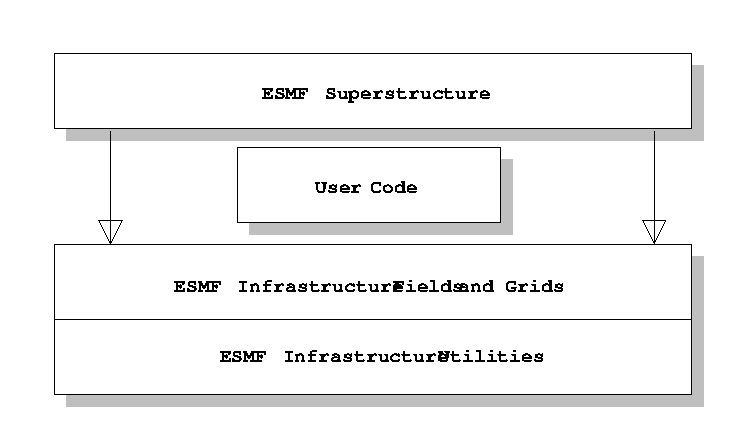
\includegraphics{esmfwich.EPS}}
\end{figure}
\end{center}

\subsection{Programming Paradigm}
A complete, executable assembly of {\bf Superstructure}, user code components and {\bf Infrastructure} collectively forms an ESMF {\it application component}.
Figure \ref{fig:ESMFApplication} shows the generic structure of an ESMF application component. 
This figure shows a single tier composition involving three components. It captures the essence of the composition based programming paradigm that 
ESMF employs, multi-tier composition is also supported in which components are recursively nested.
An application is composed by connecting together one or more
numerical simulation or other user code components within an overall ESMF based environment, figure \ref{fig:ESMFApplication} (1). User code components, figure \ref{fig:ESMFApplication} (3), are written
or modified to fit within the ESMF environment that envelopes
the user code components and that supports a unified high-level {\bf Superstructure} for connecting data and control flows between 
components. A foundation-level {\bf Infrastructure} is also provided, figure \ref{fig:ESMFApplication} (2),
to both accelerate user code development and ensure compatibility
and consistency between components and between hardware platforms. 
\begin{center}
\begin{figure}
\caption{The ESMF programming paradigm defines how an overall application is constructed. An application is an assembly
of one or more gridded and coupler components (1). Components may make use of the ESMF {\bf Infrastructure} toolkit (2). All components,
gridded components, coupler components and the top-level application component are primarily user written (3).}
\label{fig:ESMFApplication}
\scalebox{.5}{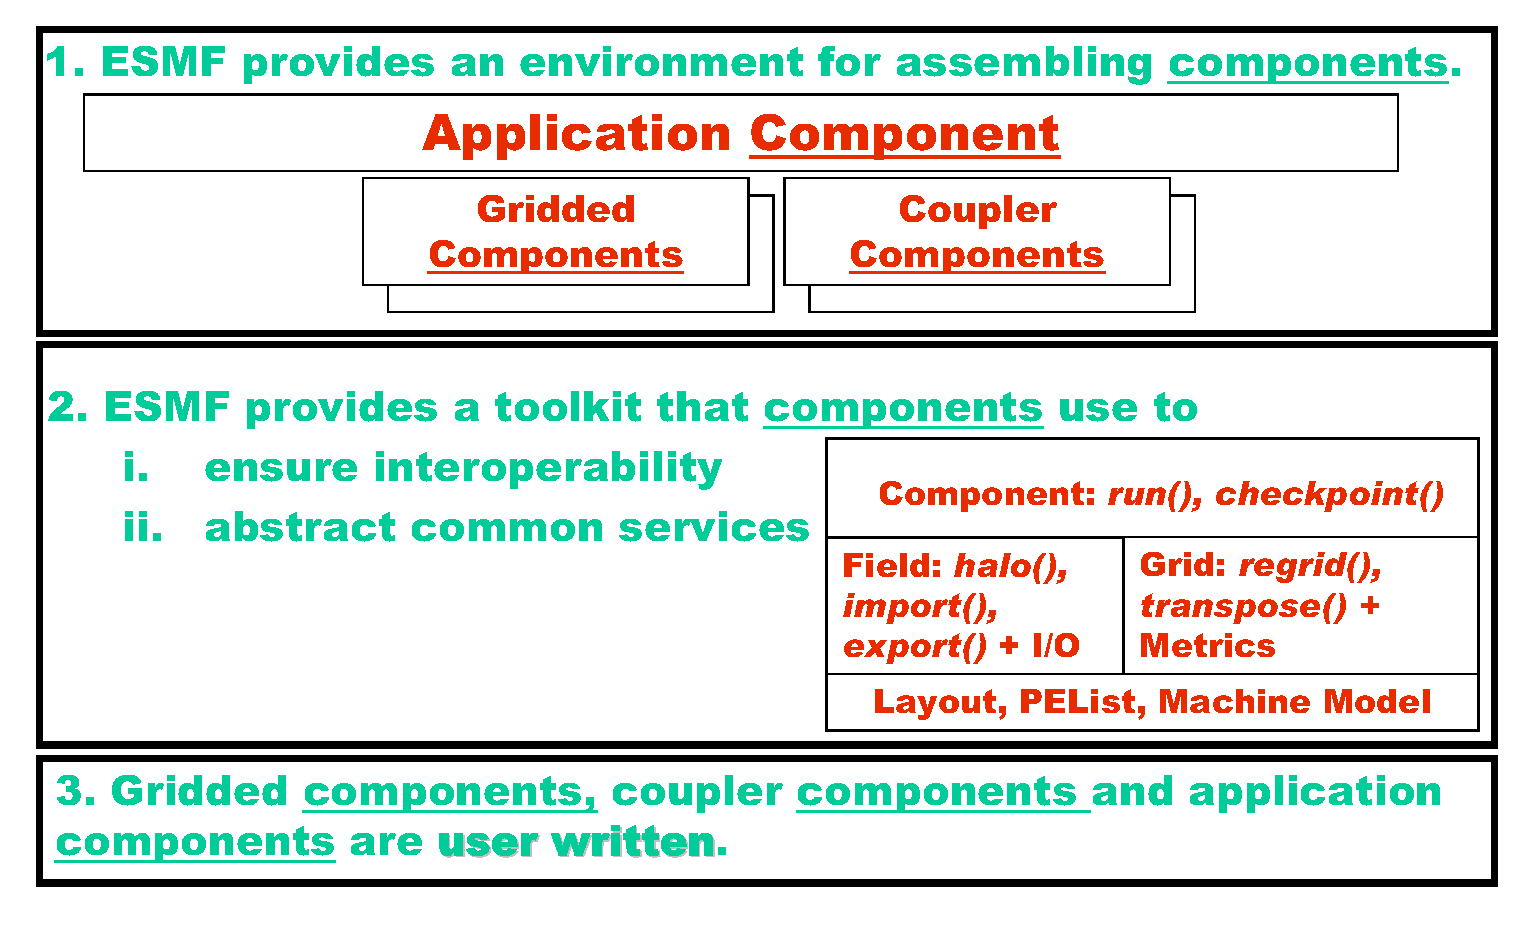
\includegraphics{ESMFprogrammingparadigm.eps}}
\end{figure}
\end{center}

\subsection{Superstructure}
\label{sec:superstructure}
The ESMF {\bf Superstructure} layers in an application furnish a unifying context within which user components are interconnected. For 
example an atmospheric model may use a particular land-surface model in calculating simulated evaporative fluxes. 
The flow of data and sequence of computation between atmospheric model term evaluations and land-surface model
term evaluations would be prescribed in the {\bf Superstructure} layer. Under ESMF user code components are constructed or adapted
to fit within this {\bf Superstructure} layer. This ensures that large components can be interchanged. There may still be issues
of physical consistency between components, but ensuring that all components comply with the requirement to fit
within an ESMF {\bf Superstructure} layer eliminates computational incompatibilities. 

The {\bf Superstructure} layer provides
the foundation for a flexible mechanism to address physical consistency between components that may use different dimensions or units to represent the
same quantity or that may partition physical data differently. Classes called {\it Gridded Components}, 
{\it Coupler Components}, {\it Import States} and {\it Export States} are used within the {\bf Superstructure} layer
to achieve this flexibility.
We describe these classes below:

\subsubsection{Import and Export State Classes}
User code components under ESMF use special interface objects for component to component data exchanges. These objects are 
of type Import State and Export State. These special types support a variety of methods that allow user code components 
to, for example, fill an export state object with data to be shared with other components or query an import state object to 
determine its contents. In keeping with the overall requirements for high-performance it is permitted for Import State and
Export State contents to use references or pointers to component data, so that costly data copies of potentially
very large data structures can be avoided where possible. The content of an Import State and an Export State is 
self-describing, so that different standards can be applied to content labeling depending on the 
by a suite of components.

\subsubsection{Interface Standards}
The Import State and Export State abstractions are designed to be flexible enough
that ESMF does not need to mandate a single standard for fields. For example ESMF does not prescribe the units
of quantities exported or imported, instead it provides mechanics to describe the units, memory layout, grid coordinates 
of the fields in Import States and Export States.  This allows the ESMF software to support a range of different policies for
physical fields. The interoperability experiments that we are using to demonstrate ESMF make use of the emerging
CF standards \cite{ref:CF} for describing physical fields. This is a policy choice for that set of experiments. The ESMF 
software itself can support arbitrary conventions for labeling and characterizing the content of Import and 
Export States.

\subsubsection{Gridded Component Class}
The Gridded Component class is used to for a user component that takes in one Import State and produces one
Export State, both based on the same discrete grid. Examples of Gridded Components are major Earth system 
model components such as land-surface models, ocean models, atmospheric models and sea-ice models. Components 
used for linear algebra manipulations in a state-estimation or data-assimilation optimization procedure are also 
created as Gridded Components. In general the Import State and the Export State of a Gridded Component will 
use the same base discrete grid.

\subsubsection{Coupler Component Class}
The other top-level component class supported in the current ESMF architecture is a Coupler Component class.
This class is used for components that take one or more Import States as input and map them through
spatial and temporal interpolation or extrapolation onto an output Export State. In a Coupler Component
it is often the case that the output Export State is on a different base discrete grid to that of
the Import State(s). The role of Coupler Components is generally mapping the Export States from one or
more Gridded Components to the Import State of another Gridded Component. For example, in a coupled
ocean-atmosphere simulation a Couple Component would be used to map a set of sea-surface fields 
in an ocean model to appropriate planetary boundary layer fields in an atmospheric model.
\subsubsection{Flexible data and control flow}
Import States, Export States, Gridded Components and Coupler Components can be arrayed flexibly
within a {\bf Superstructure} layer. Using these constructs it is possible to configure a set of concurrently
executing Gridded Components joined through a single Coupler Component of the style shown in figure 
\ref{fig:hubspoke}. Is is also possible to configure a set of sequentially executing components with multiple
pair-wise Coupler Components defined to support individual Gridded Component to Gridded 
Component mappings independently, figure \ref{fig:point2point}.

\begin{figure}
\caption{ESMF can support configurations with a single central Coupler Component. In this case inputs from all Gridded 
Components are transferred and regrided between all components in one place. The block arrows show how the 
Coupler Component 
(symbolized by the star icon) must take inputs from all Gridded Components (symbolized by the model output images) 
and return data to all Gridded Components.}
\label{fig:hubspoke}
\scalebox{0.7}{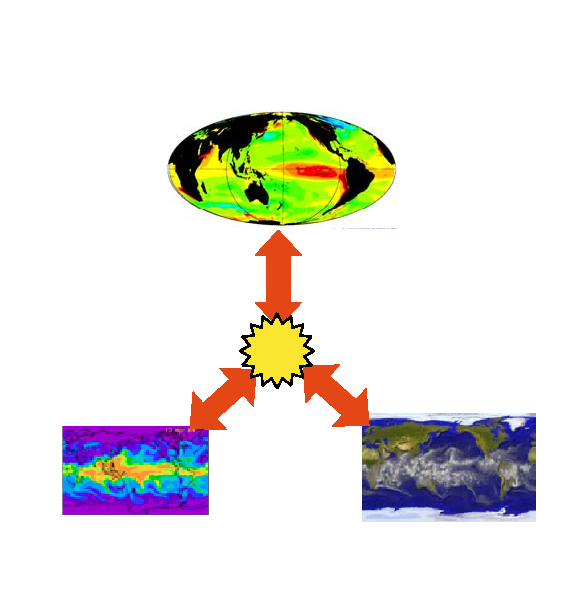
\includegraphics{couplings_hub_and_spoke.eps}}
\end{figure}

\begin{figure}
\caption{ESMF also supports configurations with multiple point to point Coupler Components. 
These take inputs from one Gridded
Component and transfer and regrid the data for passing to another Gridded Component. The block arrows show the
flow of data between point to point pairings of Coupler Components (symbolized by the star icons) and Gridded 
Components (symbolized by the model output images).}
\label{fig:point2point}
\scalebox{0.7}{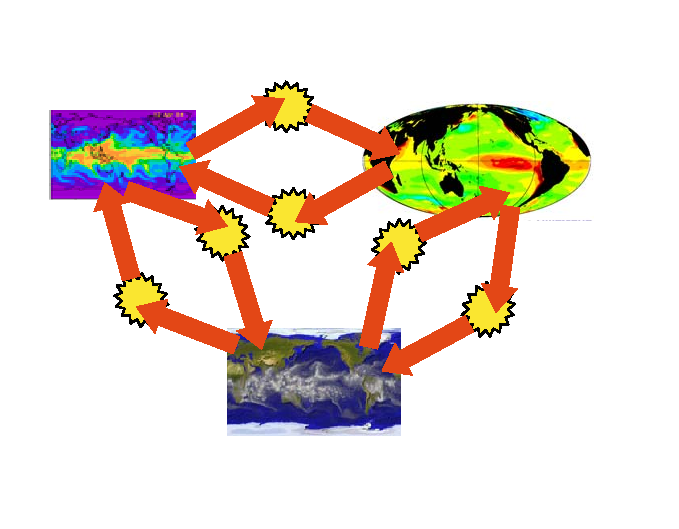
\includegraphics{couplings_pt_to_pt.eps}}
\end{figure}

The set of {\bf Superstructure} abstractions allows flexible data-flow and control between components. However, 
components will often use different discrete grids, and time-stepping components may march forward with different time
intervals. In a parallel compute environment different components may be distributed in a different manner on the
underlying compute resources. The ESMF {\bf Infrastructure} layer provides elements to manage this complexity.

\subsection{Infrastructure}
\label{sec:infrastructure}
Figure \ref{fig:threecomponents} illustrates three Gridded Components that use three different grids being coupled together. In 
order to achieve this coupling several steps beyond defining {\bf Superstructure} Import State and Export State objects to act
as data conduits are required. Coupler Components are required that can map between the different
grids, this mapping may also involve mapping between different units and/or memory layout conventions for the fields that
pass between components. In a parallel compute environment the Coupler Components may also be required to map between different 
domain decompositions. In order to advance in time correctly the separate Gridded Components must have compatible notions
of time. Approaches to parallelism within the Gridded Components must also be compatible. The {\bf Infrastructure} layer
contains a set of classes that address these issues and assist in managing overall system complexity. We describe
these classes below:

\begin{figure}
\caption{Schematic showing the coupling of components that use different discrete grids and different time-stepping. 
In this example component {\it NCAR Atmosphere} might use a spectral grid based on spherical harmonics, component
{\it GFDL Ocean} might use a latitude-longitude grid but with a patched decomposition that does not include
land masses and component {\it NSIPP Land} might use a mosaic based grid for representing vegetation patchiness
and a catchment area based grid for river routings. The {\bf Infrastructure} layer contains tools to help develop 
software for coupling between components on different grids, mapping between components with different distributions in a 
multi-processor compute environment and to synchronize events between components with different time-stepping intervals 
and algorithms.  }
\label{fig:threecomponents}
\scalebox{0.5}{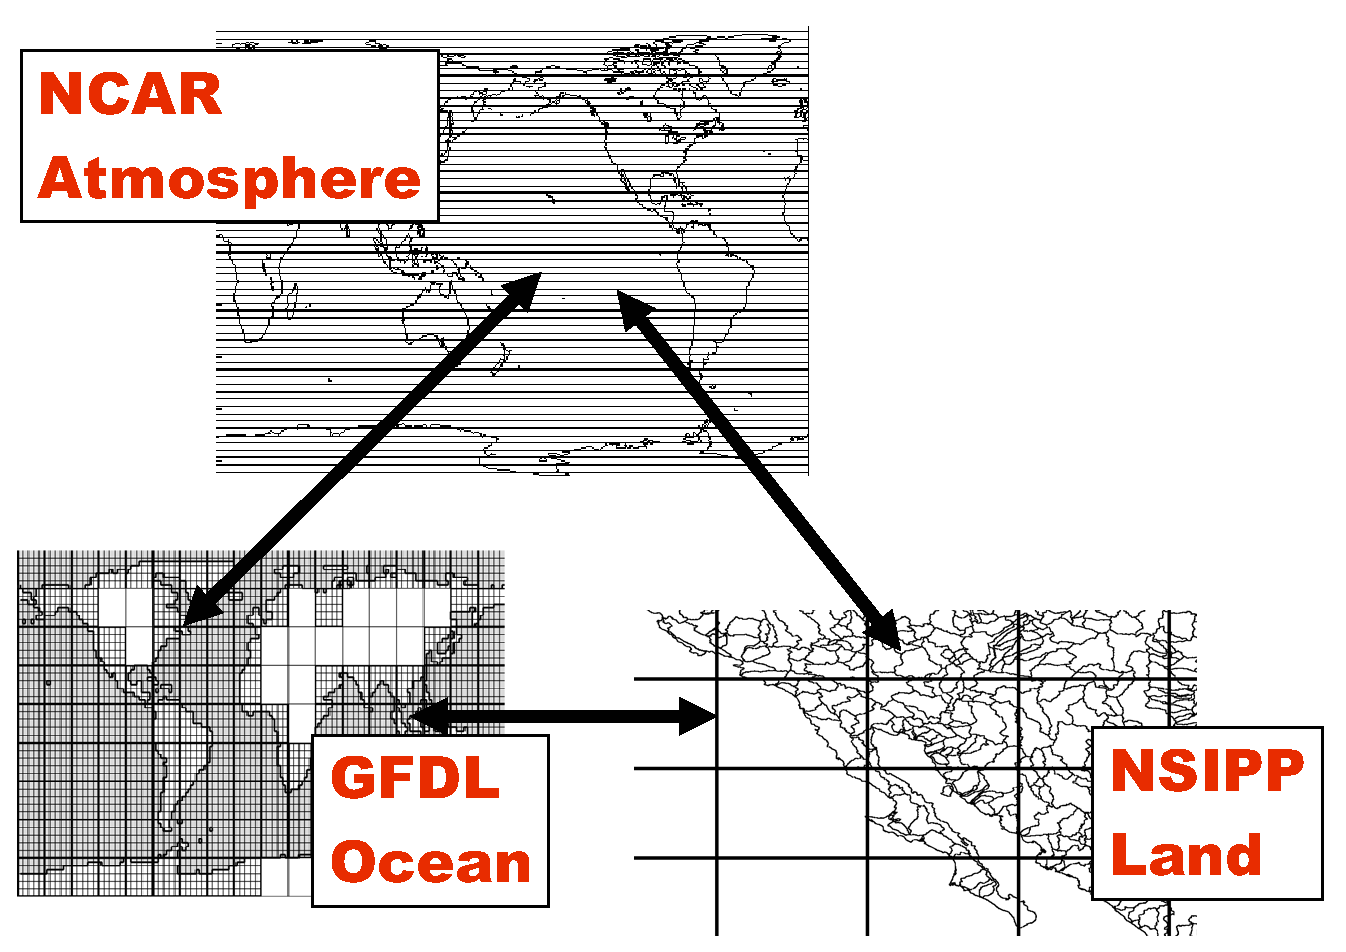
\includegraphics{regrid.eps}}
\end{figure}

\subsubsection{Field and Array Classes}
The {\it Field} and {\it Array} classes contain data together with descriptive
physical and computational attribute information. The physical attributes include information that describes the units
of the data. The computational attributes include information on the layout in memory of the field data. The Field class
is primarily geared toward structured data. A comparable class called {\it Location Stream} provides a self-describing
container for unstructured observational data streams.

\subsubsection{Physical Grid Class}
The {\it Physical Grid} class is an extensible class that holds discrete grid information. It has subtypes that allow
it to serve as a container for the full range of different physical grids that might arise in a coupled system.
In the example in figure \ref{fig:threecomponents} objects of type Physical Grid would hold grid information for
each of the spectral grid, the latitude-longitude grid, the mosaic grid and the catchment grid. 

\subsubsection{Regrid Class}
The {\it Regrid} class is an extensible class that allows conservative remapping between a field on one physical grid
to a field on a different physical grid \cite{ref:SCRIP}. It supports precomputation of grid interpolation weights and allows user selectable
corrections for global or local conservation requirements. Regrid is designed to be scalable on parallel platforms.
When mapping between grids
the Regrid class utilizes the Physical Grid object and Field and Array objects.

\subsubsection{Distributed Grid Class}
The {\it Distributed Grid} class is used to represent the decomposition of a data structure into sub-domains, typically for
parallel processing purposes. The class is designed to support a generalized ``ghosting'' for tiled 
decompositions of finite difference, finite volume and finite element codes. 

\subsubsection{Time and Calendar Management Class}
To support synchronization between components {\it Time} and {\it Calendar} classes along with an associated
{\it Clock} class are provided. These classes allow Gridded and Coupler Component processing
to be latched to a common controlling clock.

\subsubsection{I/O Classes}
The {\bf Infrastructure} layer defines a set of {\it I/O} classes for storing and retrieving Field and Grid information
to and from persistent storage. The I/O classes support a range of standard formats including binary I/O and netCDF, HDF5 and
GRIB based I/O.

\subsubsection{Communication Class}
To provide a mechanism for ensuring performance portability ESMF defines a {\it Communication} class. This class provides a set of
high-level platform independent interfaces to performance critical parallel processing communication routines. These routines can be tuned
to specific platforms to ensure optimal parallel performance on many platforms. The Communication class includes reduction
operations, transpose or redistribution operations and halo or ghost operations.

\subsubsection{Logging and Profiling Class}
The {\it Logging} and {\it Profiling} classes are designed to aid in managing the complexity of multi-component applications. They provide
ESMF with a unified mechanism for notification messages, for timing and counting events.







%\section{ESMF Technical Overview}
% $Id$

\section{Compiling and Linking User Code against an ESMF Installation}
\label{sec:Use}
% $Id$

Building user applications against an ESMF installation requires that the 
compiler and linker be able to find the appropriate ESMF header, module and 
library files. If this procedure has been documented by the installer of the 
ESMF library on your system then follow the directions given. Otherwise it is up 
to the user to determine and provide the required compiler and linker flags. 
Every ESMF installation provides a file named {\tt esmf.mk} that contains the 
relevant information.

The location of the {\tt esmf.mk} file should be documented by the party that 
installed ESMF on the system. We recommend that a single ESMF specific 
environment variable, {\tt ESMFMKFILE}, be provided by the system that points to 
the {\tt esmf.mk} file. See section \ref{InstallESMF} for the related discussion 
aimed at the person that installs ESMF on a system.

The information in {\tt esmf.mk} is defined in form of variables. In fact, 
syntactically {\tt esmf.mk} is a makefile fragment and can be imported by an 
application specific makefile via the {\tt include} command. All the variables 
in {\tt esmf.mk} start with the "{\tt ESMF\_}" prefix to prevent conflicts. The 
information in {\tt esmf.mk} is fully specified and is not affected by any 
variables set in the user's environment.

The information defined in {\tt esmf.mk} includes Fortran compiler and linker, 
as well as C++ compiler and linker. It further includes the recommended Fortran 
and C++ specific compiler and linker flags for building ESMF applications. One 
way of using the {\tt esmf.mk} is to glean the necessary information from it. 
This information can then be used either directly on the command line when 
compiling a user application, or to hardwire the settings into the application 
specific build system. However, the recommended use of {\tt esmf.mk} is to 
include this file in the application specific makefile directly via the 
{\tt include} command.

The {\tt Makefile} template below demonstrates how a user build system can be 
constructed to leverage the {\tt esmf.mk} file. In practice, most user build 
systems will be more complex. However, this template does show that the added 
complexity introduced by using {\tt esmf.mk} is minimal. Examples of how to use 
this build system in realistic user scenarios can be found in the 
\htmladdnormallink{external demos}{http://www.earthsystemmodeling.org/users/code_examples/external_demos/external_demos.shtml}.

The advantages of using {\tt esmf.mk}, over hard coding suitable compiler and 
linker flags into the user build system directly, are robustness and portability. 
Robustness is a consequence of the fact that everything defined in {\tt esmf.mk} 
corresponds to the exact settings used during the ESMF library build 
(consistency) and during the ESMF test suite build. Using {\tt esmf.mk} thus 
guarantees that the user application is build in the exact same manner as the 
ESMF test suite applications that undergo strict regression testing before every 
ESMF release. Portability means that a user build system, which uses 
{\tt esmf.mk} in the way the template {\tt Makefile} demonstrates, will function 
as expected on any system where ESMF was successfully installed and tested, 
without the need of modifying anything. Every {\tt esmf.mk} is generated during 
a specific ESMF installation using the ESMF tested settings for the host 
platform.

\begin{verbatim}

################################################################################
### Makefile template for user ESMF application, leveraging esmf.mk mechanism ##
################################################################################

################################################################################
### Finding and including esmf.mk ##############################################

# Note: This fully portable Makefile template depends on finding environment
#       variable "ESMFMKFILE" set to point to the appropriate "esmf.mk" file,
#       as is discussed in the User's Guide.
#       However, you can still use this Makefile template even if the person
#       that installed ESMF on your system did not provide for a mechanism to
#       automatically set the environment variable "ESMFMKFILE". In this case
#       either manually set "ESMFMKFILE" in your environment or hard code the
#       location of "esmf.mk" into the include statement below.
#       Notice that the latter approach has negative impact on portability.

ifneq ($(origin ESMFMKFILE), environment)
$(error Environment variable ESMFMKFILE was not set.)
endif

include $(ESMFMKFILE)

################################################################################
### Compiler and linker rules using ESMF_ variables supplied by esmf.mk ########

.SUFFIXES: .f90 .F90 .c .C

.f90:
	$(ESMF_F90COMPILER) -c $(ESMF_F90COMPILEOPTS) $(ESMF_F90COMPILEPATHS) \
          $(ESMF_F90COMPILEFREENOCPP) $<
	$(ESMF_F90LINKER) $(ESMF_F90LINKOPTS) $(ESMF_F90LINKPATHS) \
          $(ESMF_F90LINKRPATHS) -o $@ $*.o $(ESMF_F90ESMFLINKLIBS)        

.F90:
	$(ESMF_F90COMPILER) -c $(ESMF_F90COMPILEOPTS) $(ESMF_F90COMPILEPATHS) \
          $(ESMF_F90COMPILEFREECPP) $(ESMF_F90COMPILECPPFLAGS) $<
	$(ESMF_F90LINKER) $(ESMF_F90LINKOPTS) $(ESMF_F90LINKPATHS) \
          $(ESMF_F90LINKRPATHS) -o $@ $*.o $(ESMF_F90ESMFLINKLIBS)        
        
.c:
	$(ESMF_CXXCOMPILER) -c $(ESMF_CXXCOMPILEOPTS) \
          $(ESMF_CXXCOMPILEPATHSLOCAL) $(ESMF_CXXCOMPILEPATHS) \
          $(ESMF_CXXCOMPILECPPFLAGS) $<
	$(ESMF_CXXLINKER) $(ESMF_CXXLINKOPTS) $(ESMF_CXXLINKPATHS) \
          $(ESMF_CXXLINKRPATHS) -o $@ $*.o $(ESMF_CXXESMFLINKLIBS)

.C:
	$(ESMF_CXXCOMPILER) -c $(ESMF_CXXCOMPILEOPTS) \
          $(ESMF_CXXCOMPILEPATHSLOCAL) $(ESMF_CXXCOMPILEPATHS) \
          $(ESMF_CXXCOMPILECPPFLAGS) $<
	$(ESMF_CXXLINKER) $(ESMF_CXXLINKOPTS) $(ESMF_CXXLINKPATHS) \
          $(ESMF_CXXLINKRPATHS) -o $@ $*.o $(ESMF_CXXESMFLINKLIBS)

################################################################################
### Sample targets for user ESMF applications ##################################

all: esmf_UserApplication esmc_UserApplication

esmf_UserApplication:

esmc_UserApplication:

################################################################################

\end{verbatim}


\section{Using Bundled ESMF Applications}
\label{sec:Apps}
% $Id: ESMF_apps.tex,v 1.1 2010/09/27 23:13:31 rokuingh Exp $

Where do you find the ESMF\_APPSDIR?

\htmladdnormallink{external use cases}{http://www.earthsystemmodeling.org/developers/test/euc/}


\newpage

\section{Building and Installing the ESMF}
\label{sec:TechOver}

This section goes into more detail about how to build and install the ESMF
software.

% $Id: ESMF_install.tex,v 1.22 2003/05/07 14:14:38 cdeluca Exp $

\subsection{ESMF Download Options}

Major releases of the ESMF software can be downloaded by following
the instructions on the 
the {\bf Downloads \& Documentation} page on the ESMF 
website, \htmladdnormallink{http://www.esmf.ucar.edu}{http://www.esmf.ucar.edu}.  There are two options for using the ESMF:

\begin{itemize}
\item Download a pre-built ESMF shared object library and
test applications for a particular platform.  If you choose
this approach, you can skip ahead to Section~\ref{UsingLibrary},
Using the ESMF.  
\item Download the full ESMF source code, and compile and link
the framework to any necessary system libraries.  This will
result in a shared object file (with a *.so extension)
that can be linked in with the user's code, or with the demo
{ESMF\_COUPLED\_FLOW} executable.  In this case you will need
to follow all the instructions in subsequent sections of the 
{\it Quick Start} guide, beginning with Section~\ref{InstallProcedures},
Installation.
\end{itemize}

You may find it necessary to build the ESMF yourself
if we do not offer a shared object library for the current
version of your compiler.  The compiler versions that we offer
shared objects for are noted on the download web page.

\subsection{Installation}
\label{InstallProcedures}

% $Id: ESMF_systemreq.tex,v 1.2 2004/06/22 14:17:44 nscollins Exp $

\subsubsection{System Requirements}
\label{sec:systemreq}

The following compilers and utilities are required for compiling and 
linking the ESMF software:
\begin{itemize}
\item a Fortran90 compiler and libraries;
\item a C++ compiler;
\item a MPI implementation compatible with these compilers (but see below);
\item the \htmladdnormallink{GNU make}{http://www.gnu.org/software/make/make.html} utility; 
\item the tar utility, for unpacking data files;
\item the \htmladdnormallink{GNU zip}{http://www.gnu.org/software/gzip/gzip.html} utility, for unpacking data files.
\end{itemize} 

An alternative to the MPI library is provided with the ESMF,
a single-process MPI-bypass library.  It allows applications which
use MPI to be linked but only run single process.

In order to build html and pdf version of the ESMF documentation, 
\LaTeX, the latex2html conversion utility, and the dvipdf 
utility must be installed.









\subsubsection{ESMF Environment Variables}

The following environment variables must be set:
\begin{verbatim}
  ESMF_DIR      top-level ESMF directory
  ESMF_ARCH     platform and compiler configuration
\end{verbatim}

\subsubsection{Supported Platforms}
% $Id$

% List of architectures supported.  This file is 
% meant to be included in a user doc.

The following two tables list various combinations of environment 
variable settings used by the ESMF build system. A {\tt default}
value in the compiler column indicates the vendor compiler. A {\tt mpi}
value in the comm column indicates the vendor MPI implementation.

The first table lists the exact combinations which are tested regularly and are
fully supported. The second table lists all possible combinations which are 
included in the build system.

\vspace{1ex}
{\bf Fully tested combinations}: (See \htmladdnormallink{https://www.earthsystemcog.org/projects/esmf/platforms\_8\_0\_0}{https://www.earthsystemcog.org/projects/esmf/platforms\_8\_0\_0} for the most up-to-date table of supported combinations.)
\vspace{1ex}

\begin{longtable}{lllllll}
  &{\bfseries\footnotesize ESMF\_OS} &{\bfseries\footnotesize ESMF\_COMPILER} & {\bfseries\footnotesize ESMF\_COMM} & {\bfseries\footnotesize ESMF\_ABI} &
  {\bfseries\footnotesize F90 compiler} & {\bfseries\footnotesize C++ compiler} \\

%Hera 
Cray Compute   &\tt Linux  &\tt gfortran     &\tt mpiuni,            &\tt 64 & gfortran \footnotesize 4.8.4        & g++   \footnotesize 4.8.5         \\
Cluster        &           &                 &\tt intelmpi \footnotesize (2018.0.4)&       &                                     &                                   \\
Cray Compute   &\tt Linux  &\tt intel        &\tt intelmpi \footnotesize (2018.0.4)&\tt 64 & ifort    \footnotesize 18.0.5.274   & icpc  \footnotesize 18.0.5.274    \\
Cluster        &           &                 &                       &       &                                     &                                   \\
Cray Compute   &\tt Linux  &\tt pgi          &\tt mpiuni             &\tt 64 & pgf90    \footnotesize 18.10-1 	   & pgc++ \footnotesize 18.10-1       \\
Cluster        &           &                 &\tt intelmpi \footnotesize (2018.0.4)&       &                                     &                                   \\
%Cori
Cray XC30      &\tt Unicos &\tt intel        &\tt mpi \footnotesize (cray-mpich/7.7.6) &\tt 64     & ftn/ifort \footnotesize 19.0.3.199  & CC/icpc \footnotesize 19.0.3.199  \\
%Gaea
Cray XE6       &\tt Unicos &\tt gfortran     &\tt mpi \footnotesize (cray-mpich/7.7.3) &\tt 64     & ftn/gfortran \footnotesize 5.3.0    & CC/g++  \footnotesize 5.3.0       \\
Cray XE6       &\tt Unicos &\tt intel        &\tt mpi \footnotesize (cray-mpich/7.7.3) &\tt 64     & ftn/ifort \footnotesize 16.0.3.210  & CC/icpc \footnotesize 16.0.3.210  \\
Cray XE6       &\tt Unicos &\tt pgi          &\tt mpi \footnotesize (cray-mpich/7.7.3) &\tt 64     & ftn/pgf90 \footnotesize 16.5-0      & CC/pgc++\footnotesize 16.5-0      \\
%Electra
HPE/SGI ICE X  &\tt Linux  &\tt gfortran     &\tt mpiuni           &\tt 64           & gfortran \footnotesize 6.2.0        & g++ \footnotesize 6.2.0          \\
               &           &                 &\tt mpi \footnotesize (mpt/2.14r19)&                 &                                     &                                  \\
HPE/SGI ICE X  &\tt Linux  &\tt intel        &\tt mpiuni           &\tt 64           & ifort \footnotesize 15.0.3.187      & icpc \footnotesize 15.0.3.187    \\
               &           &                 &\tt mpi \footnotesize (mpt/2.12r26)&                 &                                     &                                  \\
HPE/SGI ICE X  &\tt Linux  &\tt pgi          &\tt mpiuni           &\tt 64           & pgf90 \footnotesize 17.1-0          & pgc++ \footnotesize 17.1-0       \\
%Pleiades
HPE/SGI ICE X  &\tt Linux  &\tt gfortran     &\tt mpiuni           &\tt 64           & gfortran \footnotesize 6.2.0        & g++ \footnotesize 6.2.0          \\
               &           &                 &\tt mpi \footnotesize (mpt/2.14r19)&                 &                                     &                                  \\
HPE/SGI ICE X  &\tt Linux  &\tt intel        &\tt mpiuni           &\tt 64           & ifort \footnotesize 18.0.3.222      & icpc \footnotesize 18.0.3.222    \\
               &           &                 &\tt mpi \footnotesize (mpt/2.15r20)&                 &                                     &                                  \\
HPE/SGI ICE X  &\tt Linux  &\tt pgi          &\tt mpiuni           &\tt 64           & pgf90 \footnotesize 17.1-0          & pgc++ \footnotesize 17.1-0       \\
               &           &                 &\tt mpi \footnotesize (mpt/2.17r13)&                 &                                     &                                  \\
%Cheyenne
HPE/SGI ICE XA &\tt Linux  &\tt gfortran     &\tt mpich3 \footnotesize (3.2)     &\tt 64           & gfortran \footnotesize 6.3.0        & g++ \footnotesize 6.3.0          \\
Cluster        &           &                 &                     &                 &                                     &                                  \\
HPE/SGI ICE XA &\tt Linux  &\tt gfortran     &\tt mpich3 \footnotesize (3.2)     &\tt 64           & gfortran \footnotesize 7.2.0        & g++ \footnotesize 7.2.0          \\
Cluster        &           &                 &                     &                 &                                     &                                  \\
HPE/SGI ICE XA &\tt Linux  &\tt gfortran     &\tt openmpi \footnotesize (3.1.0)  &\tt 64           & gfortran \footnotesize 8.1.0        & g++ \footnotesize 8.1.0          \\
Cluster        &           &                 &                     &                 &                                     &                                  \\
HPE/SGI ICE XA &\tt Linux  &\tt gfortran     &\tt mpt \footnotesize (2.19)       &\tt 64           & gfortran \footnotesize 9.1.0        & g++ \footnotesize 9.1.0          \\
Cluster        &           &                 &                     &                 &                                     &                                  \\
HPE/SGI ICE XA &\tt Linux  &\tt intel        &\tt mpt \footnotesize (2.19),      &\tt 64           & ifort \footnotesize 18.0.5.274      & g++ \footnotesize 18.0.5.274     \\
Cluster        &           &                 &\tt openmpi \footnotesize (3.1.4)  &                 &                                     &                                  \\
               &           &                 &\tt intelmpi \footnotesize (2018.4.274)  &           &                                     &                                  \\
HPE/SGI ICE XA &\tt Linux  &\tt intel        &\tt mpt \footnotesize (2.19)       &\tt 64           & ifort \footnotesize 19.0.2.187      & g++ \footnotesize 19.0.2.187     \\
Cluster        &           &                 &                     &                 &                                     &                                  \\
%Summitdev
IBM Power      &\tt Linux  &\tt gfortran     &\tt mpiuni           &\tt 64           & gfortran \footnotesize 4.8.5        & g++ \footnotesize 4.8.5 \\
IBM Power      &\tt Linux  &\tt pgi          &\tt mpiuni           &\tt 64           & pgf90 \footnotesize 19.7-0          & g++ \footnotesize 19.7-0 \\
%Eris
Mac Xeon       &\tt Darwin &\tt gfortran     &\tt mpiuni           &\tt 64           & gfortran \footnotesize 6.1.0        & g++ \footnotesize 6.1.0 \\
Mac Xeon       &\tt Darwin &\tt gfortran     &\tt openmpi \footnotesize (1.8)    &\tt 64           & gfortran \footnotesize 4.9.2        & g++ \footnotesize 4.9.2           \\
Mac Xeon       &\tt Darwin &\tt \footnotesize gfortranclang&\tt mpiuni           &\tt 64           & gfortran \footnotesize 6.1.0        & clang \footnotesize 1000.10.44.4  \\
%Catania
Mac Xeon       &\tt Darwin &\tt gfortran     &\tt mpiuni           &\tt 64           & gfortran \footnotesize 9.2.0        & g++ \footnotesize 9.2.0 \\
%Rutgers
Mac Xeon       &\tt Darwin &\tt gfortran     &\tt mpiuni,          &\tt 64           & gfortran \footnotesize 7.3.0        & g++ \footnotesize 7.3.0 \\
               &           &                 &\tt openmpi \footnotesize (2.1.5),&    &                                     &                                  \\
               &           &                 &\tt openmpi \footnotesize (3.1.3)&     &                                     &                                  \\
Mac Xeon       &\tt Darwin &\tt \footnotesize gfortranclang&\tt mpiuni           &\tt 64   & gfortran \footnotesize 7.3.0  & clang \footnotesize 902.0.39.2   \\
Mac Xeon       &\tt Darwin &\tt intel        &\tt mpiuni,          &\tt 64           & ifort \footnotesize 18.0.2.164      & ifort \footnotesize 18.0.2.164   \\
               &           &                 &\tt openmpi \footnotesize (2.1.5)&     &                                     &                                  \\
%Linux-regtest2
PC Xeon        &\tt Linux  &\tt gfortran     &\tt mpiuni,          &\tt 64           & gfortran \footnotesize 4.8.5        & g++ \footnotesize 4.8.5           \\
               &           &                 &\tt mpich3 \footnotesize (3.2.1) &     &                                     &                                   \\
PC Xeon        &\tt Linux  &\tt gfortran     &\tt mpiuni,          &\tt 64           & gfortran \footnotesize 7.3.0        & g++ \footnotesize 7.3.0           \\
               &           &                 &\tt mpich3 \footnotesize (3.2.1) &     &                                     &                                   \\
%Marktest
PC Xeon        &\tt Linux  &\tt gfortran     &\tt mpich3 \footnotesize (3.2.1)&\tt 64& gfortran \footnotesize 4.8.5        & g++ \footnotesize 4.8.5           \\
PC Xeon        &\tt Linux  &\tt gfortran     &\tt openmpi \footnotesize (3.1.1),&\tt 64& gfortran \footnotesize 8.1.0      & g++ \footnotesize 8.1.0           \\
               &           &                 &\tt mpich3 \footnotesize (3.2.1) &     &                                     &                                   \\
%Bebop
PC Xeon        &\tt Linux  &\tt gfortran     &\tt mvapich2 \footnotesize (2.3a), &\tt 64 & gfortran \footnotesize 7.1.0    & g++  \footnotesize 7.1.0          \\
Cluster        &           &                 &\tt mpich3 \footnotesize (3.2),    &                 &                                     &                     \\
               &           &                 &\tt openmpi \footnotesize (2.1.1), &                 &                                     &                     \\
               &           &                 &\tt intelmpi \footnotesize (2018.4.274)  &           &                                     &                     \\
PC Xeon        &\tt Linux  &\tt intel        &\tt mvapich2 \footnotesize (2.3) , &\tt 64 & ifort \footnotesize 18.0.5.274   & icpc  \footnotesize 18.0.5.274   \\
Cluster        &           &                 &\tt openmpi \footnotesize (3.1.3), &                 &                                     &                     \\
               &           &                 &\tt intelmpi \footnotesize (2018.4.274)  &           &                                     &                     \\
%Discover
PC Xeon        &\tt Linux  &\tt gfortran     &\tt mpiuni,   &\tt 64             & gfortran \footnotesize 4.8.1        & g++ \footnotesize 4.8.1                \\
Cluster        &           &                 &\tt mvapich2 \footnotesize (1.9),  &                 &                                     &                     \\
               &           &                 &\tt openmpi \footnotesize(1.7.2)  &                 &                                     &                      \\
PC Xeon        &\tt Linux  &\tt gfortran     &\tt mpiuni,   &\tt 64             & gfortran \footnotesize 4.9.2        & g++ \footnotesize 4.9.2                \\
Cluster        &           &                 &\tt mvapich2 \footnotesize (2.1),  &                 &                                     &                     \\
PC Xeon        &\tt Linux  &\tt intel        &\tt intelmpi \footnotesize (5.0.3.048) &\tt 64 & ifort \footnotesize 15.0.2.164 & icpc \footnotesize 15.0.2.164  \\
Cluster        &           &                 &                     &                 &                                     &                                   \\
PC Xeon        &\tt Linux  &\tt intel        &\tt mpiuni,  &\tt 64           & ifort \footnotesize 17.0.4.196      & icpc \footnotesize 17.0.4.196             \\
Cluster        &           &                 &\tt mvapich2 \footnotesize (2.3b)  &                 &                                     &                     \\
PC Xeon        &\tt Linux  &\tt intel        &\tt mvapich2 \footnotesize (2.3b)  &\tt 64 & ifort \footnotesize 17.0.4.196  & icpc \footnotesize 17.0.4.196     \\
Cluster        &           &                 &                     &                 &                                     &                                   \\
PC Xeon        &\tt Linux  &\tt intel        &\tt intelmpi \footnotesize (5.1.2.150) &\tt 64 & ifort \footnotesize 18.0.1.163  & icpc \footnotesize 18.0.1.163 \\
Cluster        &           &                 &                     &                 &                                     &                                   \\
PC Xeon        &\tt Linux  &\tt intel        &\tt openmpi \footnotesize (3.1.1)  &\tt 64 & ifort \footnotesize 18.0.3.222  & icpc \footnotesize 18.0.3.222     \\
Cluster        &           &                 &                     &                 &                                     &                                   \\
PC Xeon        &\tt Linux  &\tt intel        &\tt mpiuni,           &\tt 64           & ifort \footnotesize 18.0.5.274     & icpc \footnotesize 18.0.5.274     \\
Cluster        &           &                 &\tt intelmpi \footnotesize (18.0.5.274) &                 &                  &                                   \\
PC Xeon        &\tt Linux  &\tt nag          &\tt mpiuni           &\tt 64           & nagfor \footnotesize 6.2            & g++  \footnotesize 4.8.1          \\
Cluster        &           &                 &                     &                 &                                     &                                   \\
PC Xeon        &\tt Linux  &\tt pgi          &\tt mvapich2 \footnotesize (2.0b)  &\tt 64 & pgf90 \footnotesize 14.1-0      & pgc++ \footnotesize 14.1-0        \\
Cluster        &           &                 &                     &                 &                                     &                                   \\
PC Xeon        &\tt Linux  &\tt pgi          &\tt mpiuni,          &\tt 64           & pgf90 \footnotesize 17.5-0          & pgc++ \footnotesize 17.5-0        \\
Cluster        &           &                 &\tt openmpi \footnotesize (2.1.1)&     &                                     &                                   \\
PC Xeon        &\tt Linux  &\tt pgi          &\tt openmpi \footnotesize (2.1.1)&\tt 64& pgf90 \footnotesize 17.7-0         & pgc++ \footnotesize 17.7-0        \\
Cluster        &           &                 &                     &                 &                                     &                                   \\
PC Xeon        &\tt Linux  &\tt pgi          &\tt openmpi \footnotesize (3.1.1)&\tt 64& pgf90 \footnotesize 18.5-0         & pgc++ \footnotesize 18.5-0        \\
Cluster        &           &                 &                     &                 &                                     &                                   \\
%Jet
PC Xeon        &\tt Linux  &\tt intel        &\tt intelmpi \footnotesize (2018.4.274)&\tt 64& ifort \footnotesize 18.0.5.274 & icpc \footnotesize 18.0.5.274   \\
Cluster        &           &                 &                     &                 &                                     &                                   \\
PC Xeon        &\tt Linux  &\tt pgi          &\tt mpiuni           &\tt 64           & pgf90 \footnotesize 18.10-1         & pgc++ \footnotesize 18.10-1       \\
Cluster        &           &                 &\tt mvapich2 \footnotesize (2.3) &     &                                     &                                   
\end{longtable}

\vspace{1ex}

{\bf All possible options}. Where multiple options exist, and the default is independent
of {\tt ESMF\_MACHINE}, the default value is in {\bf bold}:

\vspace{1ex}


\begin{longtable}{lllll}
  {\bfseries\footnotesize ESMF\_OS} &{\bfseries\footnotesize ESMF\_COMPILER} & {\bfseries\footnotesize ESMF\_COMM} & {\bfseries\footnotesize ESMF\_ABI} \\

AIX     &\tt default     &\footnotesize \tt mpiuni,{\bf mpi},user      &\tt 32, {\bf 64} \\
Cygwin  &\tt g95         &\footnotesize \tt {\bf mpiuni},mpich,mpich2,mpich3,lam,openmpi,user &\tt 32, 64 \\
Cygwin  &\tt gfortran    &\footnotesize \tt {\bf mpiuni},mpich,mpich2,mpich3,lam,msmpi,openmpi,user &\tt 32, 64 \\
Darwin  &\tt absoft      &\footnotesize \tt {\bf mpiuni},mpich,mpich2,mpich3,mvapich2,lam,openmpi,user &\tt 32, 64 \\
Darwin  &\tt g95         &\footnotesize \tt {\bf mpiuni},mpich,mpich2,mpich3,mvapich2,lam,openmpi,user &\tt 32, 64 \\
Darwin  &\tt gfortran    &\footnotesize \tt {\bf mpiuni},mpich,mpich2,mpich3,mvapich2,lam,openmpi,user &\tt 32, 64 \\
Darwin  &\tt gfortranclang &\footnotesize \tt {\bf mpiuni},mpich,mpich2,mpich3,mvapich2,lam,openmpi,user &\tt 32, 64 \\
Darwin  &\tt intel       &\footnotesize \tt {\bf mpiuni},mpich,mpich2,mpich3,mvapich2,intelmpi,lam,openmpi,user &\tt 32, 64 \\
Darwin  &\tt intelclang  &\footnotesize \tt {\bf mpiuni},mpich,mpich2,mpich3,intelmpi,lam,openmpi,user &\tt 32, 64 \\
Darwin  &\tt intelgcc    &\footnotesize \tt {\bf mpiuni},mpich,mpich2,mpich3,intelmpi,lam,openmpi,user &\tt 32, 64 \\
Darwin  &\tt nag         &\footnotesize \tt {\bf mpiuni},mpich,mpich2,mpich3,mvapich2,lam,openmpi,user &\tt 32, 64 \\
Darwin  &\tt pgi         &\footnotesize \tt {\bf mpiuni},mpich,mpich2,mpich3,mvapich,mvapich2,lam,openmpi,user &\tt 32, 64 \\
Darwin  &\tt xlf         &\footnotesize \tt mpiuni,{\bf mpi},mpich,mpich2,mpich3,lam,openmpi,user &\tt 32 \\
Darwin  &\tt xlfgcc      &\footnotesize \tt mpiuni,{\bf mpi},mpich,mpich2,mpich3,lam,openmpi,user &\tt 32 \\
IRIX64  &\tt default     &\footnotesize \tt mpiuni,{\bf mpi},user     &\tt 32, {\bf 64} \\
Linux   &\tt absoft      &\footnotesize \tt {\bf mpiuni},mpich,mpich2,mpich3,mvapich2,lam,openmpi,user &\tt 32, 64 \\
Linux   &\tt absoftintel &\footnotesize \tt {\bf mpiuni},mpich,mpich2,mpich3,lam,openmpi,user &\tt 32, 64  \\
Linux   &\tt g95         &\footnotesize \tt {\bf mpiuni},mpich,mpich2,mpich3,mvapich2,lam,openmpi,user &\tt 32, 64, \\
        &                &                              &\tt ia64\_64, \\
        &                &                              &\tt x86\_64\_32, \\
        &                &                              &\tt x86\_64\_small, \\
        &                &                              &\tt x86\_64\_medium \\
Linux   &\tt gfortran    &\footnotesize \tt {\bf mpiuni},mpi,mpt,mpich,mpich2,mpich3,mvapich2, &\tt 32, 64, \\
        &                &\footnotesize \tt intelmpi,lam,openmpi,user                          &\tt ia64\_64, \\
        &                &                              &\tt x86\_64\_32, \\
        &                &                              &\tt x86\_64\_small, \\
        &                &                              &\tt x86\_64\_medium \\
Linux   &\tt gfortranclang &\footnotesize \tt {\bf mpiuni},mpi,mpt,mpich,mpich2,mpich3,mvapich2, &\tt 32, 64, \\
        &                & \footnotesize \tt lam,openmpi,user                                    &\tt ia64\_64, \\
        &                &                              &\tt x86\_64\_32, \\
        &                &                              &\tt x86\_64\_small, \\
        &                &                              &\tt x86\_64\_medium \\
Linux   &\tt intel       &\footnotesize \tt {\bf mpiuni},mpi,mpt,mpich,mpich2,mpich3,mvapich2, &\tt 32, 64, \\
        &                &\footnotesize \tt intelmpi,scalimpi,lam,openmpi,user                 &\tt ia64\_64, \\
        &                &                              &\tt x86\_64\_32, \\
        &                &                              &\tt x86\_64\_small, \\
        &                &                              &\tt x86\_64\_medium, \\
        &                &                              &\tt mic \\
Linux   &\tt intelgcc    &\footnotesize \tt {\bf mpiuni},mpi,mpt,mpich,mpich2,mpich3,mvapich2, &\tt 32, 64, \\
        &                &\footnotesize \tt intelmpi,lam,openmpi,user                          &\tt ia64\_64, \\
        &                &                              &\tt x86\_64\_32, \\
        &                &                              &\tt x86\_64\_small, \\
        &                &                              &\tt x86\_64\_medium \\
Linux   &\tt lahey       &\footnotesize \tt {\bf mpiuni},mpich,mpich2,mpich3,mvapich2,lam,openmpi,user &\tt 32, 64 \\
Linux   &\tt nag         &\footnotesize \tt {\bf mpiuni},mpich,mpich2,mpich3,mvapich2,lam,openmpi,user &\tt 32, 64 \\
Linux   &\tt nagintel    &\footnotesize \tt {\bf mpiuni},mpich,mpich2,mpich3,lam,openmpi,user &\tt 32, 64 \\
Linux   &\tt pathscale   &\footnotesize \tt {\bf mpiuni},mpich,mpich2,mpich3,lam,openmpi,user &\tt 32, 64, \\
        &                &                              &\tt x86\_64\_32, \\
        &                &                              &\tt x86\_64\_small, \\
        &                &                              &\tt x86\_64\_medium \\
Linux   &\tt pgi         &\footnotesize \tt {\bf mpiuni},mpi,mpt,mpich,mpich2,mpich3,mvapich,mvapich2 &\tt 32, 64, \\
        &                &\footnotesize \tt intelmpi,scalimpi,lam,openmpi,user &\tt x86\_64\_32, \\
        &                &                              &\tt x86\_64\_small, \\
        &                &                              &\tt x86\_64\_medium \\
Linux   &\tt pgigcc      &\footnotesize \tt {\bf mpiuni},mpich,mpich2,mpich3,lam,openmpi,user &\tt 32 \\
Linux   &\tt sxcross     &\footnotesize \tt mpiuni,{\bf mpi},user      &\tt 32  \\
Linux   &\tt xlf         &\footnotesize \tt mpiuni,{\bf mpi},user      &\tt 32  \\
MinGW   &\tt gfortran    &\footnotesize \tt {\bf mpiuni},msmpi,user    &\tt 32, 64 \\
MinGW   &\tt intel       &\footnotesize \tt {\bf mpiuni},msmpi,user    &\tt 32, 64 \\
MinGW   &\tt intelcl     &\footnotesize \tt {\bf mpiuni},msmpi,user    &\tt 32, 64 \\
OSF1    &\tt default     &\footnotesize \tt mpiuni,{\bf mpi},user      &\tt 64  \\
SunOS   &\tt default     &\footnotesize \tt mpiuni,{\bf mpi},user      &\tt 32, {\bf 64} \\
Unicos  &\tt default     &\footnotesize \tt mpiuni,{\bf mpi},user      &\tt 64  \\
Unicos  &\tt cce         &\footnotesize \tt mpiuni,{\bf mpi},user      &\tt 64  \\
Unicos  &\tt gfortran    &\footnotesize \tt mpiuni,{\bf mpi},user      &\tt 64  \\
Unicos  &\tt intel       &\footnotesize \tt mpiuni,{\bf mpi},user      &\tt 64  \\
Unicos  &\tt pathscale   &\footnotesize \tt mpiuni,{\bf mpi},user      &\tt 64  \\
Unicos  &\tt pgi         &\footnotesize \tt mpiuni,{\bf mpi},user      &\tt 64

\end{longtable}

\vspace{1ex}



% GNU make requirement.  File in build/doc
% $Id$ 

% Text about GNU make  This file is 
% meant to be included in a user doc.

GNU Make is required to build the ESMF library.  On some
systems this will be just the command \texttt{make}.  On others
it might be installed as \texttt{gmake} or \texttt{gnumake}.
This document uses {\tt make} consistently to refer to GNU Make.

Use the {\tt \verb+--+version} option with the locally available make commands
to determine which variant corresponds to GNU Make on your system. Use the
respective command when interacting with the ESMF build system, and
where this documentation uses {\tt make}.

Notice that ESMF does not utilize Autotools (configure or autoconf) or CMake.
Instead, the selection of configuration options is done by setting environment
variables before building the framework. The relevant environment variables
all begin with prefix {\tt ESMF\_}, and are discussed in detail under section
\ref{EnvironmentVariables}.


Simultaneous multiple architecture builds are supported, with
one restriction; the test cases may only be run on one platform at a time. 

\subsubsection{Building the ESMF Libraries}
\label{BuildESMF}

Build the library with the command:
\begin{verbatim}
  gmake BOPT=g  
\end{verbatim}
  for a debug version or
\begin{verbatim}
  gmake BOPT=O  
\end{verbatim}
  for an optimized version.

Build options that enable you to copy the library and *.mod files to
specified directories are explained in Section~\ref{BuildOptions}. 

\subsubsection{Building the ESMF Test Suites}
\label{BuildTestSuite}
A test suite is included with the library. Tests are provided for both MPI
and uniprocessor builds. Tests can be built both from the top ESMF directory and
the local source code directories.

\noindent The following command builds the System Tests:
\begin{verbatim}
  gmake BOPT=<g,O> [SYSTEM_TEST=NNNNN] build_system_tests
\end{verbatim}

For example:
\begin{verbatim}
  gmake BOPT=O build_system_tests
\end{verbatim}
Will build all available system tests. Specifying a specific SYSTEM\_TEST number will build only the specified system test.

\noindent The following command builds the Unit Tests:
\begin{verbatim}
  gmake BOPT=<g,O> [ESMF_EXHAUSTIVE=<ON,OFF>] build_tests
\end{verbatim}

For example:
\begin{verbatim}
  gmake BOPT=g ESMF_EXHAUSTIVE=OFF build_tests
\end{verbatim}
will build tests that verify basic correctness of the library build and installation. Turning the {\tt ESMF\_EXHAUSIVE} option {\tt ON} when building will create a more comprehensive set of tests, but, will take significantly longer to run. 

Output files from the test examples will be directed to files in:
\begin{verbatim}
  ${ESMF_DIR}/test${BOPT}/${ESMF_ARCH}
\end{verbatim}

See Section~\ref{TestingProcedures} for instruction on running ESMF tests.

\subsubsection{Building the ESMF Documentation}
\label{BuildDocumentation}

\noindent To build documentation:
\begin{verbatim}
  gmake dvi           ! Makes the dvi files.
  gmake pdf           ! Makes the pdf files.
  gmake html          ! Creates the html directory.
  gmake alldoc        ! Builds all the above documents.
\end{verbatim}

\noindent To build documentation for one module:

\noindent First change directory to the where the desired module's documentation resides;  for
example, to build the {\tt TimeMgmt} documentation start with:

\begin{verbatim}
cd ${ESMF_DIR}/src/Infrastructure/TimeMgmt/doc
\end{verbatim}

\noindent Next issue one of the following commands:
\begin{verbatim}
  gmake localdvi      ! Builds local dvi files.
  gmake localpdf      ! Builds local pdf files.
  gmake localhtml     ! Builds local html files.
  gmake localdoc      ! Builds all of the local documents.
\end{verbatim}

\noindent The output from this local documentation build is in the top level {\tt doc}
directory, as with the previous commands.









\section{Porting the ESMF}
\label{sec:TechOverPort}

This section goes into more detail about the ESMF build system and how to
port the ESMF software to new platforms.

%  $Id: ESMF_builddetail.tex,v 1.1 2003/08/26 17:40:16 flanigan Exp $


\subsection{Make System}
For most users the description of the build system in the Quick Start
section should be sufficient.  Some users, however, may wish to have a
more detailed knowledge of the make system that is used by the library
either for configuring different build options or other reasons.
\subsubsection{General Structure}

The ESMF build system is broken into two parts.  The first is the
series of makefiles located with the source code.  The second is a set
of makefile fragements files designed to be used by the source code
makefiles.  Makefile fragment files are files that contain makefile
syntax defining build rules and actions, but do not constitute a
complete build system.

The main components of the make system are:
\begin{itemize}
\item{Build directories}

There are two directories containing makefile fragment files used by
the make system.  Makefile fragment files are files that contain
makefile syntax defining build rules and variables, but do not
constitute a complete build system.

The {\tt esmf\_build} directory contains a generic makefile fragment
file common.mk that is included by the top level Makefile in the
source tree.  common.mk contains generic build system settings and
build rules used across all platforms.

The {\tt esmf\_build\_config} directory contains makefile fragments
for each supported platform defining compilers, compiler flags, and
the various other definitions that are necessary to build on each
platform.  Files can also be added to this directory for specific
machines where the build settings are different from the standards of
the architecture.  One of the files in this directory will be included
by the esmf\_build/common.mk file depending the values of the environment
variable EMSF\_ARCH and ESMF\_SITE.  See below for more details on this
topic.

\item{Environment Variables}

The three sets of source code that the build system support all need
environment variables set to point to their top level source code
directories. 

\begin{itemize}

\item{ESMF Library} The ESMF library needs ESMF\_DIR set .

\item{Implementation Report} The Implementation Report needs ESMF\_IMPL\_DIR set.  


\item{EVA Applications} An EVA source code tree does not contain a copy of the ESMF build
system.  Instead it uses a copy found in an ESMF source code tree.
ESMF\_EVA\_DIR has to be set to the top most directory of the EVA source
code.  ESMF\_DIR has to be set to the top most directory of an ESMF
source code tree.


\end{itemize}

\begin{description}

\item{ESMF\_ARCH} 
Defines current architecture. Default value is value returned by the
command uname -s.  There should be almost no reason for ESMF\_ARCH to
be set by a user.


\item{ESMF\_SITE}

If ESMF\_SITE is not set or has the value of default, default build
settings for the current machine architecture will be used.  Values
are created from a machine's name and if needed, the compiler used.
Example ESMF\_SITE values could be blackforest or jazz\_lahey.

\item{ESMF\_PREC}

Variable specifying the precession build arguments.  Value can be 32
or 64.  When possible the default value will be 64, otherwise it will
be 32.

\item{ESMF\_BOPT} 

Variable specifying that the build system use either debugging or
optimization options.  Value of g specifies the debugging options.
Value of O (capital oh) specifies optimization options.  Default value
is O.

\end{description}


\item{Top level Makefile}

The top level makefile includes the common.mk file from the {\tt
esmf\_build} directory.  Many of the commands in this Makefile spawn a recursive make
through the directory structure.

\item{Source tree Makefiles}

Each directory contains a Makefile which includes the {\tt build} common
makefiles.  These local Makefiles include defintions that allow the local files
and documents to be built.
\end{itemize}

\subsubsection{Configuration}



\subsection{Build Options}
\label{BuildOptions}

There is an install target which will copy the library and *.mod files to
specified directories.  To invoke this target use:
\begin{verbatim}
  gmake BOPT=[O,g] ESMF_LIB_INSTALL=<path for library>
                   ESMF_MOD_INSTALL=<path for *.mod files> install 
\end{verbatim}

Some users may wish for the library to be built in a directory different from 
where the source code resides.  To do this, build using:
\begin{verbatim}
   gmake ESMF_BUILD=<path> BOPT=[O,g]
\end{verbatim}

The {\tt ESMF\_BUILD} variable gives an alternate path in which to
place the libraries, *.mod files and object files.  This variable
defaults to {\tt ESMF\_DIR}.  If it is assigned another value, the
{\tt ESMF\_BUILD} variable will need to be passed as an additional
argument to the the above make commands.  (Alternatively the variable
{\tt ESMF\_BUILD} can be set in the environment (using setenv or
export) and then it need not be passed to any make calls).



\section{Validating an ESMF Build}
\label{sec:TechOver2}

This section goes into more detail about how to run the tests, which are
included with the ESMF software, to validate an ESMF build.

% $Id: ESMF_testing.tex,v 1.2 2003/03/20 20:03:11 btwomack Exp $

\section{Testing}
\label{testing}

\subsection{Description}
\label{TestDescription}
Robust high quality software is a primary goal of the ESMF development effort. To ensure that goal is met, the ESMF includes a comprehesive suite of tests. They allow test and validation of everything from individual functions to complete system tests. These test suites are used by the ESMF development team as part of their regular development process. Model developers can also use the testing suites to verify that the software was built and installed properly. It can also assist them in the debugging process when integrating user supplied model components. 

\subsubsection{Unit Test Description}
\label{UnitTestDescription}
The Unit tests provided with the ESMF library evaluate the following:
\begin{itemize}
\item correctness of individual functions
\item behavior of individual modules or classes
\end{itemize}

\subsubsection{System Test Description}
\label{SystemTestDescription}

The System tests provided with the ESMF library evaluate the following:
\begin{itemize}
\item interface agreement between parts of the system
\item behavior of the system as a whole
\end{itemize}

The current system test suite includes tests that perform layout reduction operations, redistribution-transpose, halo operations, component creation, intra-grid communication, etc. A complete description of each available system test can be found at the ESMF website on the developers page. 

\subsubsection{EVA Test Suite Description}
\label{EVATestDescription}

The ESMF VAlidation(EVA) Suite is a collection of seven codes representative of those used in climate, weather, and data assimulation. These codes are currently used for ESMF prototyping. They will eventually provide the basis for ESMF tutorial examples.

\subsection{Procedures}
\label{TestingProcedures}

The following test procedures assume that ESMF library source code has been built and installed. Please ensure that the build and install steps are completed before proceeding. See Section~\ref{InstallProcedures} for installation procedures and Section~\ref{BuildTestSuite} for information on building ESMF tests.  

\subsubsection{Running ESMF Unit Tests}
\label{RunUnitTests}

The following commands are used to build and run the unit tests provided with the ESMF:
\begin{verbatim}
        gmake BOPT=<g,O> [ESMF_EXHAUSTIVE=<ON,OFF>] tests
        gmake BOPT=<g,O> [ESMF_EXHAUSTIVE=<ON,OFF>] tests_uni
\end{verbatim}

The results of the test can be found in the following location:
\begin{verbatim}
       ${ESMF_DIR/test/test${BOPT}/${ESMF_ARCH}
\end{verbatim}

For example: 

If your esmf source files have been placed in: 
\begin{verbatim}
       /usr/local/esmf
\end{verbatim}

and your platform and compiler configuration is:
\begin{verbatim}
       Linux uni-processor using the LF95 compiler
\end{verbatim}

and you want to run a debug version of exhaustive unit tests,
then you use the command:
\begin{verbatim}
       gmake BOPT=g ESMF_EXHAUSTIVE=ON tests_uni
\end{verbatim}

and will find the results in:
\begin{verbatim}
       /usr/local/esmf/test/testg/linux_lf95/
\end{verbatim}

\subsubsection{Running ESMF System Tests}
\label{RunSystemTests}

The following commands are used to build and run the system tests:

\begin{verbatim}
        gmake BOPT=<g,O> [SYSTEM_TEST=NNNNN] system_tests
        gmake BOPT=<g,O> [SYSTEM_TEST=NNNNN] system_tests_uni
\end{verbatim}

If SYSTEM\_TEST is not specified, then all available system tests will be built and run.

The results of the test can be found in the following location:
\begin{verbatim}
       ${ESMF_DIR/test/test${BOPT}/${ESMF_ARCH}
\end{verbatim}

For example: 

If your esmf source files have been placed in your home directory:
\begin{verbatim}
       ~/esmf
\end{verbatim}

and your platform and compiler configuration is:
\begin{verbatim}
       Alpha multi-processor using the native compiler
\end{verbatim}

and you want to run an optimized version of system test number 62502,
then you use the command:
\begin{verbatim}
       gmake BOPT=O SYSTEM_TEST=62502 system_tests
\end{verbatim}

and will find the results in:
\begin{verbatim}
       ~/esmf/test/testO/alpha/62502 
\end{verbatim}

\subsubsection{Running EVA Suite Tests}
\label{RunEVATests}

The EVA Suite User's Guide (http://www.esmf.ucar.edu/esmf\_docs/EVA\_usrdoc/index.html) describes how to compile and run these codes, which can be downloaded from SourceForge (http://cvs.sourceforge.net/cgi-bin/viewcvs.cgi/esmf/eva\_src/). 





























% $Id: ESMF_examples.tex,v 1.6 2004/07/01 20:13:24 svasquez Exp $

\subsection{Running ESMF Examples}
\label{examples}


\subsubsection{Example Source Code}

Example source code for each class is found in the class's example
directory. For example, source code for the Time Manager class examples
are found in this directory:

\begin{verbatim}
        ESMF_DIR/src/Infrastructure/TimeMgr/examples/
\end{verbatim}

While the example code is formatted to be included in the documentation,
it also runs and compiles to ensure accuracy.  Examples generally 
contain simple usage of the basic methods for the class.

\subsubsection{Building and Running Examples}

The GNU makefile targets {\tt examples} and {\tt examples\_uni} build
and run programs found in a class's examples directory.  After the
examples are built, the {\tt examples} target runs the examples using
multiple processors, while {\tt examples\_uni} runs the examples on
a single processor.

These targets first build the ESMF library.

Run from ESMF\_DIR, this command will build and run all examples on
multiple processors:

\begin{verbatim}
       gmake examples
\end{verbatim}

If the command is run in an example source code directory, then only
the example from that directory will be built and run.  The examples
and output files are created in this directory:

\begin{verbatim}
       ESMF_DIR/examples/examples$ESMF_BOPT/$ESMF_ARCH.$ESMF_COMPILER.$ESMF_PREC.$ESMF_SITE/
\end{verbatim}

The name of an output file will begin with the name of the example
that created it followed by .stdout.

At the end of examples execution a script runs to analyze the results.
The script, which is written in ksh, will not run on platforms that do not support
ksh. Those platforms print out a 'Command not found' message.

The script output indicates whether there are any system test failures.
The following is a sample from the script output:

\begin{verbatim}
The following is the analysis of the run examples results:

Executable examples found:
-rwxr-xr-x   1 svasquez ncar          40059 Jul 01 13:38 ESMC_AppMainEx
-rwxr-xr-x   1 svasquez ncar          37761 Jul 01 13:38 ESMC_CplEx
-rwxr-xr-x   1 svasquez ncar          37184 Jul 01 13:35 ESMC_FieldCreateEx
-rwxr-xr-x   1 svasquez ncar          37761 Jul 01 13:38 ESMC_GCompEx
-rwxr-xr-x   1 svasquez ncar          37945 Jul 01 13:34 ESMC_RouteEx
-rwxr-xr-x   1 svasquez ncar          50065 Jul 01 13:29 ESMF_AlarmEx
-rwxr-xr-x   1 svasquez ncar          65842 Jul 01 13:38 ESMF_AppMainEx
-rwxr-xr-x   1 svasquez ncar          46810 Jul 01 13:35 ESMF_ArrayCommEx
-rwxr-xr-x   1 svasquez ncar          47233 Jul 01 13:33 ESMF_ArrayCreateEx
-rwxr-xr-x   1 svasquez ncar          44725 Jul 01 13:31 ESMF_ArrayDataMapEx
-rwxr-xr-x   1 svasquez ncar          47227 Jul 01 13:33 ESMF_ArrayGetEx
-rwxr-xr-x   1 svasquez ncar          41291 Jul 01 13:30 ESMF_ArraySpecEx
-rwxr-xr-x   1 svasquez ncar          52829 Jul 01 13:36 ESMF_BundleCreateEx
-rwxr-xr-x   1 svasquez ncar          43091 Jul 01 13:36 ESMF_BundleDataMapEx
-rwxr-xr-x   1 svasquez ncar          44084 Jul 01 13:29 ESMF_CalendarEx
-rwxr-xr-x   1 svasquez ncar          46960 Jul 01 13:29 ESMF_ClockEx
-rwxr-xr-x   1 svasquez ncar          55286 Jul 01 13:38 ESMF_CplEx
-rwxr-xr-x   1 svasquez ncar          43151 Jul 01 13:33 ESMF_DELayoutEx
-rwxr-xr-x   1 svasquez ncar          57465 Jul 01 13:37 ESMF_FieldCommEx
-rwxr-xr-x   1 svasquez ncar          51113 Jul 01 13:35 ESMF_FieldCreateEx
-rwxr-xr-x   1 svasquez ncar          45436 Jul 01 13:34 ESMF_FieldDataMapEx
-rwxr-xr-x   1 svasquez ncar          50319 Jul 01 13:35 ESMF_FieldWriteEx
-rwxr-xr-x   1 svasquez ncar          55643 Jul 01 13:38 ESMF_GCompEx
-rwxr-xr-x   1 svasquez ncar          46331 Jul 01 13:33 ESMF_GridCreateEx
-rwxr-xr-x   1 svasquez ncar          42787 Jul 01 13:28 ESMF_LogErrEx
-rwxr-xr-x   1 svasquez ncar          53913 Jul 01 13:37 ESMF_RegridEx
-rwxr-xr-x   1 svasquez ncar          57428 Jul 01 13:34 ESMF_RouteEx
-rwxr-xr-x   1 svasquez ncar          54225 Jul 01 13:38 ESMF_StateEx
-rwxr-xr-x   1 svasquez ncar          45652 Jul 01 13:29 ESMF_TimeEx
-rwxr-xr-x   1 svasquez ncar          47977 Jul 01 13:29 ESMF_TimeIntervalEx
-rwxr-xr-x   1 svasquez ncar          42537 Jul 01 13:31 ESMF_VMAllFullReduceEx
-rwxr-xr-x   1 svasquez ncar          47314 Jul 01 13:31 ESMF_VMComponentEx
-rwxr-xr-x   1 svasquez ncar          42502 Jul 01 13:31 ESMF_VMDefaultBasicsEx
-rwxr-xr-x   1 svasquez ncar          40901 Jul 01 13:31 ESMF_VMGetMPICommunicatorEx
-rwxr-xr-x   1 svasquez ncar          44418 Jul 01 13:31 ESMF_VMScatterVMGatherEx
-rwxr-xr-x   1 svasquez ncar          42668 Jul 01 13:31 ESMF_VMSendVMRecvEx
-rwxr-xr-x   1 svasquez ncar          40765 Jul 01 13:37 ESMF_XformEx

All of the executable examples should have a corresponding stdout file.
If not, it's an indication that the examples ere not executed, or that it failed to execute.

Examples stdout files found: 
-rw-rw-r--   1 svasquez ncar            620 Jul 01 13:38 ESMC_AppMainEx.stdout
-rw-rw-r--   1 svasquez ncar            488 Jul 01 13:38 ESMC_CplEx.stdout
-rw-rw-r--   1 svasquez ncar            332 Jul 01 13:35 ESMC_FieldCreateEx.stdout
-rw-rw-r--   1 svasquez ncar            490 Jul 01 13:39 ESMC_GCompEx.stdout
-rw-rw-r--   1 svasquez ncar            590 Jul 01 13:34 ESMC_RouteEx.stdout
-rw-rw-r--   1 svasquez ncar           6233 Jul 01 13:30 ESMF_AlarmEx.stdout
-rw-rw-r--   1 svasquez ncar           3460 Jul 01 13:39 ESMF_AppMainEx.stdout
-rw-rw-r--   1 svasquez ncar            342 Jul 01 13:35 ESMF_ArrayCommEx.stdout
-rw-rw-r--   1 svasquez ncar           6632 Jul 01 13:33 ESMF_ArrayCreateEx.stdout
-rw-rw-r--   1 svasquez ncar           2837 Jul 01 13:31 ESMF_ArrayDataMapEx.stdout
-rw-rw-r--   1 svasquez ncar           6617 Jul 01 13:33 ESMF_ArrayGetEx.stdout
-rw-rw-r--   1 svasquez ncar            514 Jul 01 13:30 ESMF_ArraySpecEx.stdout
-rw-rw-r--   1 svasquez ncar           1189 Jul 01 13:36 ESMF_BundleCreateEx.stdout
-rw-rw-r--   1 svasquez ncar           2106 Jul 01 13:36 ESMF_BundleDataMapEx.stdout
-rw-rw-r--   1 svasquez ncar            378 Jul 01 13:30 ESMF_CalendarEx.stdout
-rw-rw-r--   1 svasquez ncar           1536 Jul 01 13:30 ESMF_ClockEx.stdout
-rw-rw-r--   1 svasquez ncar           2228 Jul 01 13:39 ESMF_CplEx.stdout
-rw-rw-r--   1 svasquez ncar           7019 Jul 01 13:33 ESMF_DELayoutEx.stdout
-rw-rw-r--   1 svasquez ncar            658 Jul 01 13:37 ESMF_FieldCommEx.stdout
-rw-rw-r--   1 svasquez ncar           2768 Jul 01 13:36 ESMF_FieldCreateEx.stdout
-rw-rw-r--   1 svasquez ncar           4997 Jul 01 13:35 ESMF_FieldDataMapEx.stdout
-rw-rw-r--   1 svasquez ncar            923 Jul 01 13:36 ESMF_FieldWriteEx.stdout
-rw-rw-r--   1 svasquez ncar           2518 Jul 01 13:39 ESMF_GCompEx.stdout
-rw-rw-r--   1 svasquez ncar            755 Jul 01 13:34 ESMF_GridCreateEx.stdout
-rw-rw-r--   1 svasquez ncar            327 Jul 01 13:29 ESMF_LogErrEx.stdout
-rw-rw-r--   1 svasquez ncar            435 Jul 01 13:37 ESMF_RegridEx.stdout
-rw-rw-r--   1 svasquez ncar            638 Jul 01 13:34 ESMF_RouteEx.stdout
-rw-rw-r--   1 svasquez ncar           3474 Jul 01 13:38 ESMF_StateEx.stdout
-rw-rw-r--   1 svasquez ncar            563 Jul 01 13:29 ESMF_TimeEx.stdout
-rw-rw-r--   1 svasquez ncar            778 Jul 01 13:29 ESMF_TimeIntervalEx.stdout
-rw-rw-r--   1 svasquez ncar            684 Jul 01 13:32 ESMF_VMAllFullReduceEx.stdout
-rw-rw-r--   1 svasquez ncar           7476 Jul 01 13:32 ESMF_VMComponentEx.stdout
-rw-rw-r--   1 svasquez ncar           3116 Jul 01 13:31 ESMF_VMDefaultBasicsEx.stdout
-rw-rw-r--   1 svasquez ncar            397 Jul 01 13:31 ESMF_VMGetMPICommunicatorEx.stdout
-rw-rw-r--   1 svasquez ncar           1806 Jul 01 13:32 ESMF_VMScatterVMGatherEx.stdout
-rw-rw-r--   1 svasquez ncar           1479 Jul 01 13:32 ESMF_VMSendVMRecvEx.stdout
-rw-rw-r--   1 svasquez ncar            822 Jul 01 13:37 ESMF_XformEx.stdout

Example stdout files of zero length indicate that the example
did not run because it failed to compile or it failed to execute. 

The following examples passed: 
ESMF_AlarmEx.stdout
ESMF_AppMainEx.stdout
ESMF_ArrayCommEx.stdout
ESMF_ArrayCreateEx.stdout
ESMF_ArrayDataMapEx.stdout
ESMF_ArrayGetEx.stdout
ESMF_ArraySpecEx.stdout
ESMF_BundleCreateEx.stdout
ESMF_BundleDataMapEx.stdout
ESMF_CalendarEx.stdout
ESMF_ClockEx.stdout
ESMF_CplEx.stdout
ESMF_DELayoutEx.stdout
ESMF_FieldCommEx.stdout
ESMF_FieldCreateEx.stdout
ESMF_FieldDataMapEx.stdout
ESMF_FieldWriteEx.stdout
ESMF_GCompEx.stdout
ESMF_GridCreateEx.stdout
ESMF_LogErrEx.stdout
ESMF_RegridEx.stdout
ESMF_RouteEx.stdout
ESMF_StateEx.stdout
ESMF_TimeEx.stdout
ESMF_TimeIntervalEx.stdout
ESMF_VMAllFullReduceEx.stdout
ESMF_VMComponentEx.stdout
ESMF_VMDefaultBasicsEx.stdout
ESMF_VMGetMPICommunicatorEx.stdout
ESMF_VMScatterVMGatherEx.stdout
ESMF_VMSendVMRecvEx.stdout
ESMF_XformEx.stdout


No examples Failed.


\end{verbatim}




%\section{Looking Ahead:  How to Adapt Applications for ESMF}

%\section{Glossary}

This glossary defines terms used in Earth system modeling to describe 
parallel computer architectures, grids and grid decompositions, and 
numerical and computational methods.  While some of the concepts in 
the glossary may eventually appear as computational objects, many 
will not.  The goal here is not to define a framework design or an 
object model but simply to achieve a common language.

\begin{description}

\item[Accumulator] \label{glos:Accumulator} A facility for collecting and 
  averaging data values.  Generally accumulators are associated with 
  temporal averaging, although they might be associated with 
  other weighted averaging operations.    
  
\item[Address space] \label{glos:ASP}A standard term to refer to the memory
  seen by a computer program that it can write to directly using
  simple language primitives. 

\item[Alarm] \label{glos:Alarm} An event 
  that occurs at a particular time (or set of times).  It is like an
   alarm on a real alarm clock except that in order to determine whether 
it is "ringing", an alarm is "read" by an explicit application action.

\item[Addressable node] \label{glos:Anode} A set of processors that are
  capable of addressing the same set of blocks of physical memory.

\item[Application] \label{glos:Application} A coherent computational 
  entity run 
  as a single executable or set of communicating executables.  It 
  typically consists of a set of interacting components.

\item[Background grid] \label{glos:BackGrid} 
  A background grid associates each point in a location stream with a 
  location on a grid. A single grid cell may contain zero or more location 
  stream points.  

\item[Bundle] \label{glos:Bundle} A bundle refers to a set of fields that 
  are associated with the same physical grid and distributed in a similar 
  fashion across the same physical axes.  Fields within a bundle may be
  staggered differently and may have different dimensions.

\item[Calendar interval] \label{glos:CalInt} A period of time specified
in calendar-based units that may be used to increment or decrement time instants.  
One year and three months is an example of a calendar interval.  Since 
mathematical operations involving calendar intervals may be ambiguously 
defined -- for example, incrementing January 31 in the Gregorian calendar by 
one month -- default behavior must be carefully specified.  

\item[Cell] \label{glos:Cell} A physical location that is specified by both 
  its extent (vertices) and nominal central location, and is associated with 
  a single integer index value or a set of integer index values ( e.g.
  (i) for 1-d, (i,j) for 2-d, (i,j,k) for 3d ).

\item[Clock] \label{glos:Clock} A clock tracks the passage of time and 
reports the current time instant, like a real clock.  However, most clocks 
used in ESMF components have a key difference to a real clock. Clocks 
in an ESMF component are generally stepped forward by the component, as an 
explicitly coded time step within the overall component.

\item[Component] \label{glos:Component} A large-scale computational entity 
  associated with a particular physical process or computational function, 
  such as a land model.  Components may be generic or user-supplied.  
  See also gridded component, coupler component.

\item[Compute resource] \label{glos:CompResource} Something that appears as a
  physical or virtual computer resource. Example of compute resources
  are a CPU, a network connection, a communication API, a protocol, a 
  particular network fabric or a piece of computer memory. 

\item[Coupler component] \label{glos:Coupler}
  A component that includes all data and actions needed to enable 
  communication between two or more other components.

\item[Data dependency] \label{glos:DataDep} The property of a computational
  operator that defines the data indices required to perform
  the computation at a point.  For instance, a forward differencing
  operation in X at $(i,j)$ has a dependency on $(i+1,j)$.

\item[Data transpose] \label{glos:DataTranspose} Rearrangement of data arrays 
  between two distributed grids sharing the same global domain.

\item[Day of year] \label{glos:DayOfYear} The day number in the calendar year. 
January 1 is day 1 of the year. Day of year expressed in a floating point 
format is used to express the day number plus the time of day. 
For example, assuming a Gregorian calendar:

\begin{tabular}{ll}
{\bf date}              & {\bf day of year} \\
\hline 
10 January 2000, 6Z     & 10.25 \\
31 December 2000, 18Z   & 366.75 
\end{tabular}

\item[DE] \label{glos:DE} 
Short for decomposition element.

\item[Decomposition element (DE)] \label{glos:Decomp_Element}
A decomposition element is a virtual portion of a computer 
associated with a processing element and an address space.  A DE may 
be associated with an MPI process or a thread.  Layouts 
assign a topology to decomposition elements.

\item[Distributed grid] \label{glos:DistGrid}
  A distributed grid defines the decomposition of the global index space 
  across the layout and methods on the indexed data.

\item[Distribution] \label{glos:Distribution} The function that expresses
the relationship between the indices in a distributed grid and the elements 
in a layout.  

\item[Domain decomposition] \label{glos:DomainDecomp} The act of grid 
  distribution: creating a layout; and associating gridpoints with the layout. 
  The dimensionality of the domain decomposition is the dimensionality of 
  the associated layout.

\item [Exact] \label{glos:Exact} The word exact is used
to denote entities, such as time instants and time intervals, for which truncation-free arithmetic is required. 

\item[Exchange grid] \label{glos:ExchangeGrid} A grid whose vertices are
formed by the intersection of the vertices of two overlying grids.  Each 
cell in the exchange grid overlies exactly one cell in each grid of the 
exhange.

\item[Exchange packets] \label{glos:EP} The data exchanged by components.  
  Exchange packets may or may not contain contiguous data, and may contain 
  both field and other forms of data.

\item[Exclusive domain] \label{glos:ExcDomain} The set of indices whose 
  data is exclusively and definitively updated by a particular PE.

\item[Executable] \label{glos:Exec} 
  A parallel program that is under independent control by the operating 
  system.

\item[Export state] \label{glos:ExportState} The data and 
  metadata that a component can make available for exchange 
  with other components. This may be data at a physical boundary 
  (e.g land-atmosphere interface) or in other cases, it might be the 
  entire model state.  See also restart state, import state.

\item[Field] \label{glos:Field} A field is a physical quantity
  defined within a region of space.  A field includes a grid 
  and any metadata necessary for a full description of the field data.

\item[Functionality Class] \label{glos:FuncClass}
A functionality class is a body that accomplishes a given function, such
as I/O. It may contain several different classes or extend over multiple
framework layers. Functionality classes are described in the ESMF Architecture
Document.

\item[Generic component] \label{glos:GenericTrans} A generic component
  is one supplied by the framework.  The user is not expected to 
  customize or otherwise modify it.  See also user component.

\item[Generic transform] \label{glos:GenericTrans} A generic transform 
  is a operation supplied by the framework, for example, a method 
  that converts gridded data from one supported physical grid and/or 
  decomposition to another using a specified technique.  See also user 
  transform.

\item[Global physical grid] \label{glos:GlobPhysGrid} 
  A global physical grid contains physical information about the entire, 
  undecomposed domain.  No distributed grid need be associated with a global 
  physical grid.  

\item[Global domain] \label{glos:GlobDomain}
  The global range of indices of data points.

\item[Global reduction] \label{glos:GlobReduction} 
  Reduction operations (sum, max, min, etc.) on
  data defined on a distributed grid.  See also global broadcast.

\item[Global broadcast] \label{glos:GlobBroadcast}
  Scatter operations on data defined on a distributed grid.
  See also global reduction.

\item[Grid] \label{glos:Grid} The discrete division of space associated with
  a particular coordinate system.  A grid contains all physical grid and memory 
  organization information (via distributed grid and layout) required to manipulate 
  fields, as well as to create and execute grid transforms. 

\item[Grid metrics] \label{glos:GridMetrics} Terms relating measurements 
  in index space to physical grid quantities like distances and areas.

\item[Grid staggering] \label{glos:GridStagger} 
  A descriptor of relative locations
  of scalar and vector data on a structured grid. On different
  staggered grids, vector data may lie at cell faces or vertices,
  while scalar data may lie in the interior. The staggered locations
  are often written in a notation like $(i+\frac12,j+\frac12)$ to
  describe the offset of a corner with respect to the cell $(i,j)$.

\item[Grid topology] \label{glos:GridTopo} Description of data 
  connectivities in index space.

\item[Grid union] \label{glos:GridUnion} The formation of a new grid
  by taking the union of the vertices of two input grids. 

\item[Gridded component] \label{glos:GridComp}
  A component that is associated with one or more grids.  No requirements 
  may be placed on the physical content of a gridded component's data or 
  on the nature of its computations. 

\item[Halo] \label{glos:Halo} 
  The points in the data domain outside the local domain. 

\item[Halo update] \label{glos:HaloUpdate}
  Halo points are associated with other PEs'
  local domains, and the halo update operation involves
  synchronization of some or all halo points with other PEs. 

\item[Import state] \label{glos:ImportState} The data and metadata 
  that a component requires from other components in order to run.  
  See also export state, restart state.

\item[Index] \label{glos:Index} An integer value associated with a set
  of coordinates that describe a cell or location in physical space.

\item[Index space] \label{glos:IndexSpace} The space implied 
  by a set of indices.  An index space has a defined dimensionality and 
  connectivity.

\item[Index space location] \label{glos:IndexSpaceloc} 
  A location within index space.  A index space location may be fractional.
  See also physical location.

\item[Layout] \label{glos:Layout} A layout specifies a PE list, 
  decomposition strategy (thread and process), and the dimensionality 
  and connectivity of the decomposition.  Multiple distributed 
  grids may be defined per layout.

\item[Local domain] \label{glos:LocalDomain} This includes the exclusive 
  domain, as well as the points with whom the exclusive points have data 
  dependencies.

\item[Local physical grid] \label{glos:LocPhysGrid} The portion of a 
  physical grid associated with a local domain.  

\item[Location stream] \label{glos:LocStream} A list of
  locations with no assumed relationship between these locations.  The
  elements of a location stream are assumed to share the same data
  items and metadata, though some elements may have blank entries for
  particular data or attributes.

\item[Logically rectangular grid] \label{glos:RecGrid} A grid in 
  which sequential indices are physically adjacent, and in which the 
  extent of each index is independent of the other indices.

\item[Loose bundle] \label{glos:LooseBundle} A loose bundle consists of 
  fields whose data is not contiguous in memory.

\item[Machine model] A generic representation of the computing 
  platform architecture.

\item[Mask] \label{glos:Mask} A field marking a span within a larger grid.

\item[Memory domain] \label{glos:MemDomain} The portion of memory 
  associated with an local domain.  The memory domain is always at least 
  as large as the local domain.

\item[Memory node] \label{glos:Mnode} A set of processors
  sharing equal flat access to a block of physical memory.

\item[MPMD] \label{glos:MPMD} Multiple Program Multiple Datastream.
  Multiple executables, any of which could itself be an SPMD
  executable, executing independently within an application.

\item [No-leap calendar] \label{glos:NoLeap} Every year uses the same months 
and days per month as in a non-leap year of a Gregorian calendar.

\item[Packed bundle] \label{glos:PackedBundle} A packed bundle is arranged
  so that field data is contiguous in memory.

\item[Partition] \label{glos:Partition} In a multi-threaded application, the subset of a
  computational domain that is associated with a logically independent
  sequence of operations. The logical independence requirement is so
  that partitions may be scheduled as separable concurrent tasks.

\item[PE] \label{glos:PE} Short for processing element.

\item[PE list] \label{glos:PElist} A list of processor IDs associated 
  with a component.  See also layout.

\item[Physical grid] \label{term:PhysGrid} 
  A physical grid contains a variety of information
  on the location in physical space and physical metrics (area,
  grid lengths, etc.) of various grid points.

\item[Physical location] \label{glos:PhysLoc} The point in physical space 
  to which data pertain. 

\item[Platform] \label{glos:Platform} 
  The processor hardware, operating system, compiler and
  parallel library that together form a unique compilation target.

\item[Processing element (PE)] \label{glos:Processing_Element}
A processing element is associated with a single hardware processor.  It may
have a framework ID that is different than its vendor-assigned ID.  

\item[Processing node] \label{glos:Pnode} A set of processors to which an
  operating system scheduler is capable of assigning to a single job.

\item[Restart state] \label{glos:RestartState} The component 
  data that 
  is needed for an exact restart. This can include, in addition to 
  a physical state,  time information, static field data,
  metadata and control information. 

\item[Scheduler] \label{glos:Scheduler} An operating system component 
  that assigns system
  resources (processors, memory, CPU time, I/O channels, etc.) to
  executables.

\item[Span] \label{glos:Span} The physical extent associated with a grid.

\item[SPMD] \label{glos:SPMD} Single Program Multiple Datastream. 
  A single executable, possibly with many 
  components (representing for example the atmosphere, the ocean, 
  land surface) executing serially or concurrently.

\item [System time] \label{SysTime}Time spent doing system tasks such as I/O or in system calls.  May also
include time spent running other processes on a multiprocessor system.

\item [Time instant] \label{glos:TimeInstant}
Generic name for an absolute time and date specification. A time instant is made 
up of a time and date and an associated calendar. It may include a time zone.
``Jan 3rd 1999, 03:30:24.56s, UTC'' is one example of a time instant.

\item [Time interval] \label{glos:TimeInterval} A time interval is the
period between any two time instants, measured in units, such as days, 
seconds, and fractions of a second, that are not associated with a specific
calendar.  Time intervals may be negative.  The periods 2 days and 10 seconds, 
86400 and 1/3 seconds and 31104000.75 seconds are all examples of time intervals.  
Mathematical operations such as addition, multiplication and subdivision 
can be applied to time intervals.

\item [User component] \label{UserComp} A component that is customized or
written by the user.  See also generic component.

\item [User time] \label{UserTime} Processor time actually spent executing a process's code.

\item[User transform] \label{glos:UserTrans} A user-supplied 
  method that is used to extend framework capabilities beyond generic 
  transforms.  

\item [Wall clock time] \label{WallClockTime} Elapsed real-world time (i.e. difference between start time minus
stop time).

\end{description}










































\end{document}







